\documentclass[11pt,xcolor={dvipsnames}]{beamer}
\usepackage{beamerthemeshadow}
\usetheme{Frankfurt}
\usepackage{graphics}
\usepackage{mathtools}  
\mathtoolsset{showonlyrefs}
\usepackage{float}
\usepackage{transparent}
\usepackage{subfigure} % Use multiple figures
\usepackage{wrapfig}
\usepackage{pifont}
\usepackage{multirow}
\usepackage{hyperref}
\usepackage{url}
\usepackage{caption}




% additional usepackage{beamerthemeshadow} is used

\usepackage{beamerthemeshadow}

\usepackage[T1]{fontenc}
\usepackage{accents}

\renewcommand*{\thefootnote}{\fnsymbol{footnote}}
\definecolor{links}{HTML}{2A1B81}
\hypersetup{colorlinks,linkcolor=,urlcolor=links}

\newcommand*{\bbar}[1]{\accentset{[-]}{#1}}
\newcommand*{\pbar}[1]{\accentset{(-)}{#1}}

\setbeamertemplate{footline}{\insertframenumber/\inserttotalframenumber}

\newenvironment<>{varblock}[2][.9\textwidth]{%
  \setlength{\textwidth}{#1}
  \begin{actionenv}#3%
    \def\insertblocktitle{#2}%
    \par%
    \usebeamertemplate{block begin}}
  {\par%
    \usebeamertemplate{block end}%
  \end{actionenv}}
  
\pdfpageattr {/Group << /S /Transparency /I true /CS /DeviceRGB>>} 

\title{{\Large \textbf{Search for long-lived neutral particles decaying to photons at 8 TeV}\\
\vspace{2mm}
\normalsize Approval of EXO-14-017}}
\author{Alberto Ocampo, Michael Sigamani, \textbf{Ward Van Driessche}}
\date{\today} 
\institute{University of Ghent}

\begin{document}

\begin{frame}
\titlepage
\begin{columns}
\begin{column}{6cm}
\centering
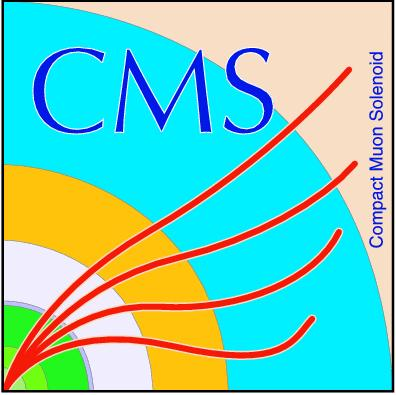
\includegraphics[height=0.15\textheight]{cms.jpeg}
\end{column}
\begin{column}{6cm}
\centering

\includegraphics[height=0.15\textheight]{logo.jpg}
\end{column}
\end{columns}
\end{frame} 


\begin{frame}[noframenumbering]
\frametitle{Outline}
\vspace{-2mm}
\scriptsize
\tableofcontents[hideallsubsections]
\end{frame}

\section[Intro]{Introduction}
\label{introdu}
\begin{frame}
\frametitle{\insertsection}

%\centering
%\textbf{\large Search for displaced photons.}

\begin{columns}
\begin{column}{6cm}
\begin{block}{}
\setbeamertemplate{itemize items}[ball]
\begin{itemize}
\item \textcolor{Red}{\textbf{GMSB signal model:}} 
\setbeamertemplate{itemize items}[default]
\begin{itemize}
\item $ \tilde{\chi}^0_1\rightarrow \gamma$ + Gravitino.
%\item Gauge interaction responsible for \textbf{soft SUSY breaking} in MSSM.
\item Neutralino is NLSP
\item Gravitino is LSP
\end{itemize}
\vspace{3mm}
\setbeamertemplate{itemize items}[ball]
%\item $E^{miss}_T$ because of Gravitino when assuming conserved R-parity.
\item \textcolor{Red}{\textbf{Two free parameters:}}
\begin{itemize}
%\setbeamertemplate{itemize items}[default]
\item Mean lifetime of $\widetilde{\chi}^0_1$ ($c\tau$)
\item \textcolor{Green}{SUSY breaking scale ($\Lambda$)}
\end{itemize}
\end{itemize}
\end{block}

\begin{itemize}
\item AN (v13): \href{http://cms.cern.ch/iCMS/jsp/openfile.jsp?tp=draft&files=AN2013_421_v13.pdf}{ \textcolor{black}{\textbf{Click here}}}
\item PAS (v11): \href{http://cms.cern.ch:80/iCMS/analysisadmin/get?analysis=EXO-14-017-pas-v11.pdf}{ \textcolor{black}{\textbf{Click here}}} 
\item Twiki: \href{https://twiki.cern.ch/twiki/bin/viewauth/CMS/DisplacedPhotonsWithConversions8TeV}{ \textcolor{black}{\textbf{Click here}}}
\item CADI: \href{http://cms.cern.ch/iCMS/analysisadmin/cadilines?line=EXO-14-017}{ \textcolor{black}{\textbf{Click here}}}  
\end{itemize}

\end{column} 

\begin{column}{6cm}
\centering
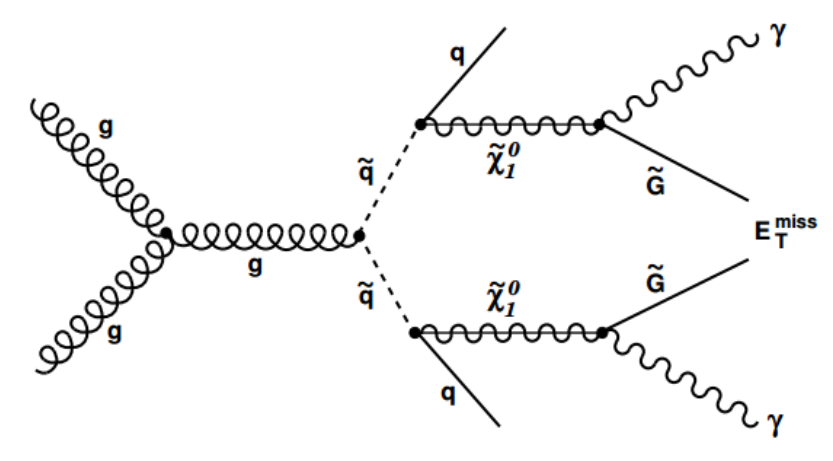
\includegraphics[width=0.9\textwidth]{Feynman1.png}\\ 
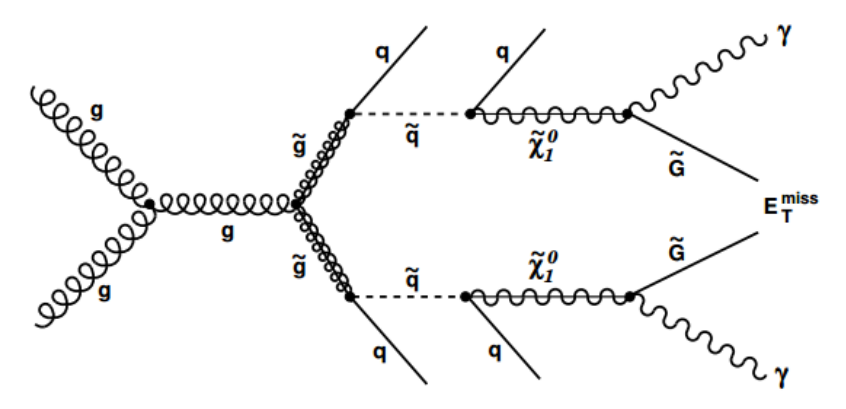
\includegraphics[width=0.9\textwidth]{Feynman2.png}\\
\end{column}
\end{columns}
\end{frame}




\subsection{Related analyses}
\begin{frame}
\frametitle{\insertsubsection}
\vspace{-4mm}
\begin{columns}
\begin{column}{6.0cm}
\vspace{-4mm}
\begin{block}{\footnotesize Using conversions at 7 TeV (2.1 fb$^{-1}$)}
\begin{itemize}
\begin{scriptsize}
\item $\geq 2$ photons ($p_T > 45$ GeV)
\item $\geq 2$ jets ($p_T >$ 80 \& 50 GeV)
\item $E^{miss}_T > 30$ GeV 
\item \textcolor{Red} {EXO-11-067: JHEP (2012)} 
\end{scriptsize}
\end{itemize}
\end{block}
\end{column}
\hspace{1mm}
\begin{column}{5.9cm}
\vspace{-4mm}
\begin{block}{\footnotesize Using ECAL timing at 7 TeV (4.8 fb$^{-1}$)}
\begin{itemize}
\begin{scriptsize}
\item $\geq 1$ photon ($p_T \geq 100$ GeV)
\item $\geq 3$ jets ($p_T >$ 35 GeV)
\item \textcolor{Red} {EXO-11-035: PLB (2013)} 
\end{scriptsize}
\end{itemize}
\end{block}
\end{column}
\end{columns}

\begin{columns}
\begin{column}{5.8cm}
\vspace{-4mm}
\begin{exampleblock}{\footnotesize Using ECAL timing at 8 TeV (19.1 fb$^{-1}$)}
\begin{footnotesize}
\begin{itemize}
\item $\geq 1$ photon ($p_T > $ 80 \& 45 GeV) 
\item $\geq 2$ jets ($p_T > $ 35 GeV)
\item $E^{miss}_T > 60$ GeV
\end{itemize} 
\end{footnotesize}
\end{exampleblock}
\end{column}
\hspace{-3mm}
\begin{column}{6.2cm}
\begin{itemize}
\begin{small}
\setbeamertemplate{itemize items}[ball]
\item \textcolor{Blue}{\textbf{This analysis: A reboot of EXO-11-067 at 8 TeV}} 
\begin{itemize}
\setbeamertemplate{itemize items}[default]
\item Both 8 TeV analyses are complementary (next slide)
\item Both 8 TeV analyses are pre-approved + aiming for PAS
\end{itemize}
\end{small}
\end{itemize}
\end{column}
\end{columns}
\end{frame}

\subsubsection{limit plots}
\begin{frame}
\frametitle{\insertsubsection}
\begin{columns}
\begin{column}{6.7cm}
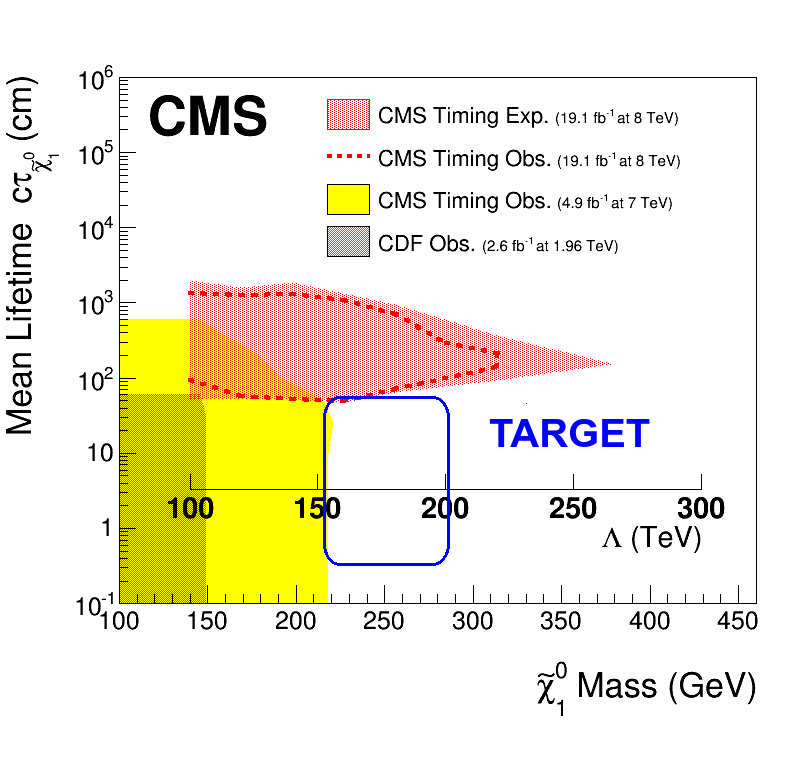
\includegraphics[width=\textwidth]{limit2D_noresult.png}\\
\hspace{-5mm}
\end{column}
\begin{column}{5.5cm}
\begin{itemize}
\begin{large}
\item Plot exclusion as 2D plot in $c\tau$ and $\Lambda$ 
\begin{itemize}
\setbeamertemplate{itemize items}[default]
\item \textcolor{Yellow}{ECAL timing - 7 TeV}
\item \textcolor{Red}{ECAL timing - \\ 8 TeV (not yet approv.)}
\item \textcolor{blue}{Conversions - 8 TeV}
\end{itemize}
\setbeamertemplate{itemize items}[ball]
\item Conversions are sensitive to lifetimes between $c\tau$ = 0.4 - 100 cm 
\vspace{3mm}
\item Generate signal MC between $\Lambda = 140 - 180$ TeV
\end{large}
\end{itemize}
\end{column}
\end{columns}
\end{frame}



\subsection{MC Samples}
\begin{frame}
\frametitle{\insertsubsection}
\begin{columns}
\begin{column}{3.5cm}
\begin{exampleblock}{\begin{center}M$_{\chi^0_1} = 198$ GeV\end{center}}
\begin{center}$\Lambda = 140$ TeV\end{center}
\end{exampleblock}
\end{column}
\begin{column}{3.5cm}
\begin{alertblock}{\begin{center}M$_{\chi^0_1} = 228$ GeV\end{center}}
\begin{center}$\Lambda = 160$ TeV\end{center}
\end{alertblock}
\end{column}
\begin{column}{3.5cm}
\begin{block}{\begin{center}M$_{\chi^0_1} = 257$ GeV\end{center}}
\begin{center}$\Lambda = 180$ TeV\end{center}
\end{block}
\end{column}
\end{columns}
\begin{figure}
\centering
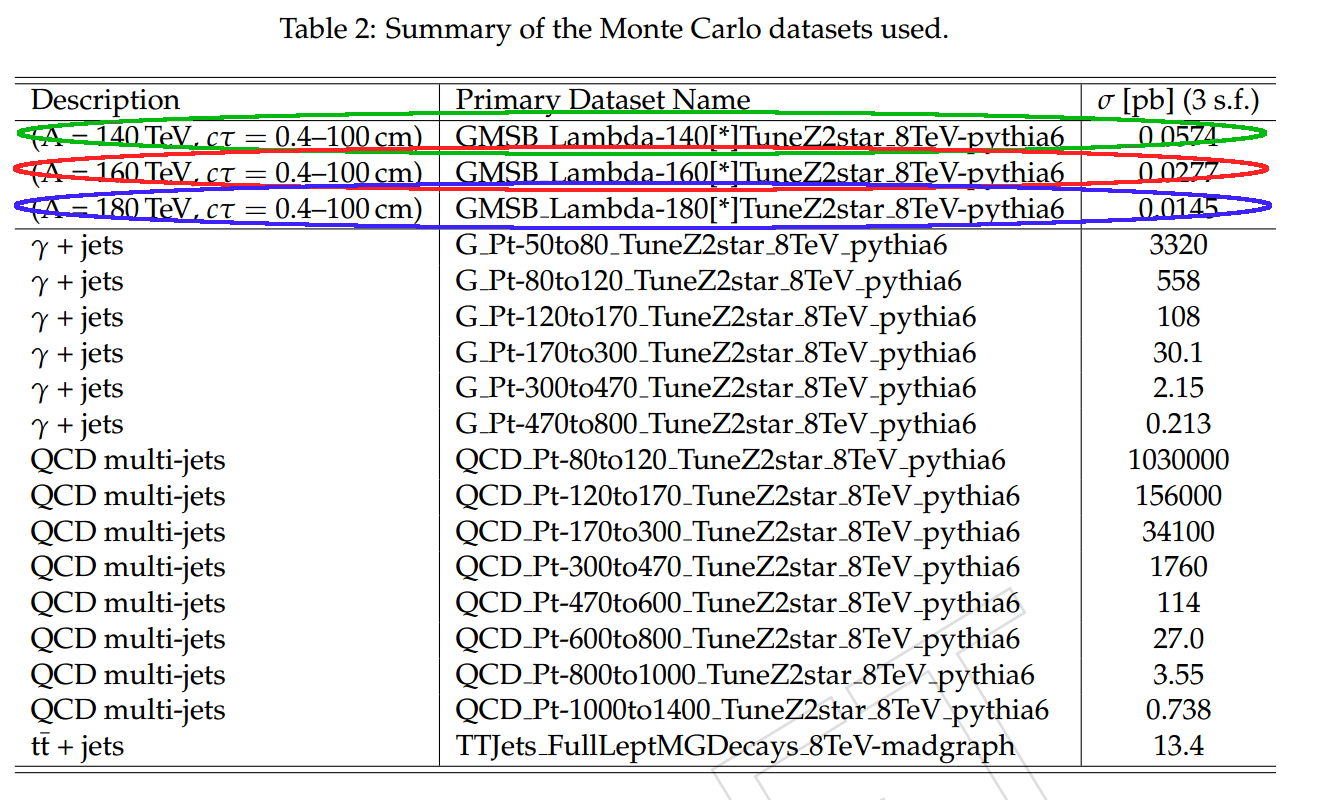
\includegraphics[width=0.7\textwidth]{table.png}\\
\end{figure}
\vspace{-5mm}
\begin{center}\normalsize \textbf{AN-13-421: Table 2}\end{center}
\vspace{-2mm}
\begin{itemize}
\item \textbf{Generate 1M signal events}
\end{itemize}

\end{frame}



\section{Data samples}

\subsection{Data/Trigger}
\begin{frame}
\frametitle{\insertsection}
%\includegraphics[width=0.95\textwidth]{datasamples.png}\\
%\vspace{-3mm}


\centering
\begin{alertblock}{\small Use Official JSON}
\begin{itemize}
\begin{scriptsize}
%\item LHC 2012 at 8 TeV: $\int L dt = 19.3$ fb$^{-1}$
\item Cert\_190456-208686\_8TeV\_22Jan2013ReReco\_Collisions12\_JSON.txt
\end{scriptsize}
\end{itemize}
\end{alertblock}
\begin{block}{\small Trigger}
\begin{itemize}
\begin{scriptsize}
\item \textbf{HLT\_DoublePhoton40\_CaloIdL\_Rsq0p035 (unprescaled):}
\begin{itemize}
\setbeamertemplate{itemize items}[default]
\begin{scriptsize}
\item Select photon $p_T > $ 50 GeV
\item Select offline photon ID to be on plateau of trigger efficiency 
\end{scriptsize}
\end{itemize}
\end{scriptsize}
\end{itemize}
\end{block}

\begin{scriptsize}
\begin{table}[!ht]
\begin{center}
\begin{tabular}{l|l|c}
\hline
\hline
 Run range &  Primary Dataset Name  & Lumi [fb$^{-1}$] \\
\hline

 190456--193621  &   /Photon/Run2012A-22Jan2013-v1/AOD        &  0.87 \\
 193834--196531  &  /DoublePhoton/Run2012B-22Jan2013-v1/AOD   &  4.43 \\
 198022--203742  & /DoublePhoton/Run2012C-22Jan2013-v2/AOD    &  7.15 \\
 203777--208686  & /DoublePhoton/Run2012D-22Jan2013-v1/AOD    &  7.30 \\

\hline
& Total & 19.7\\
\hline \hline
\end{tabular}
\end{center}
\begin{center}\normalsize \textbf{AN-13-421: Table 1}\end{center}
\end{table}
\end{scriptsize}


\end{frame}



\section[Obj. ID.]{Object ID}

\subsection{Photon Selection}
\begin{frame}
\frametitle{\insertsection: \insertsubsection}
\begin{block}{\insertsubsection}
\begin{itemize}
\item Use loose E/$\gamma$ photon ID \href{https://twiki.cern.ch/twiki/bin/viewauth/CMS/CutBasedPhotonID2012}{(TWIKI)}.
\begin{itemize}
\setbeamertemplate{itemize items}[default]
\item Isolation sums with cone size $\Delta R = 0.3$:
\setbeamertemplate{itemize items}[circle]
\begin{itemize}

\item $\sum E_{\textrm{Photon}} < 0.005 \cdot E_T + 1.3$ GeV
\item $\sum E_{\textrm{Neutral Hadron}} < 0.04 \cdot E_T + 3.5$ GeV
\item $\sum E_{\textrm{Charged Hadron}} < 2.6$ GeV

\end{itemize}
\setbeamertemplate{itemize items}[default]
\item H/E $<$ 0.05
\item $\sigma_{\eta \eta} \le$ 0.012
\item Conversion Safe Electron Veto
\end{itemize}
\setbeamertemplate{itemize items}[ball]
\item \textcolor{ForestGreen}{The $p_T$ of leading photon $\geq$ 85 GeV}
\item \textcolor{ForestGreen}{All other photons $p_T$ $\geq$ 50 GeV}
\item \textcolor{ForestGreen}{$|\eta| <$ 1.47}
\item \textcolor{ForestGreen}{0.15 $\le S_{minor} \le$ 0.3}
\end{itemize}
\end{block}
\end{frame}






\begin{frame}
\frametitle{\insertsection: \insertsubsection}
Reject events where electrons or jets fake the signature of a photon:
\begin{center}
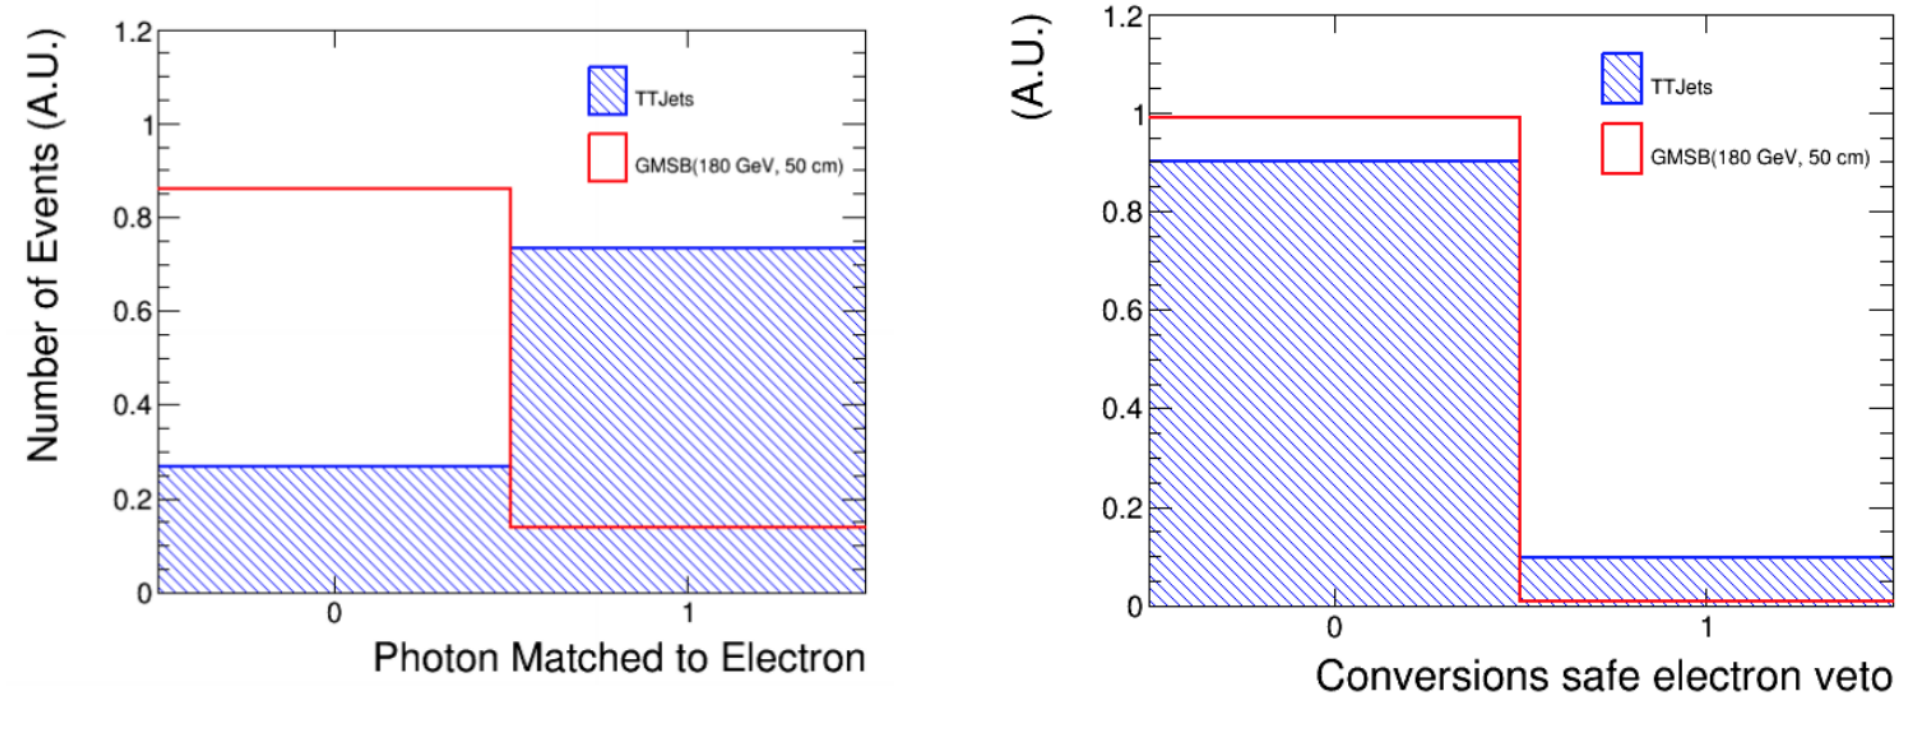
\includegraphics[width=0.8\textwidth]{electronveto.png}
\end{center}
\begin{itemize}

\item Reduce $t\bar{t}$-bar contribution by ``cleaning'' the photon objects.
\item Veto photons (left) or conversions (slide \ref{convselec}) found within a $\Delta R$ of 0.25 of a GSF electron.
\item Our ``home-made'' veto is more efficient than Conversion Safe Electron Veto (CSEV) that rejects electrons (right).
\end{itemize}
\end{frame}


\subsection{Jet Selection}
\begin{frame}
\frametitle{\insertsection: \insertsubsection}
\vspace{-2mm}
\begin{columns}
\begin{column}{6cm}
\begin{block}{\insertsubsection}
\begin{itemize}
\item Use Recommended Loose Jet ID \href{https://twiki.cern.ch/twiki/bin/view/CMS/JetID}{(TWIKI)}
\setbeamertemplate{itemize items}[default]
\begin{itemize}
\item Charged EM energy fraction (CEF) $<$ 0.99
\item Neutral hadronic energy fraction (NHF) $<$ 0.99
\item Neutral EM energy fraction (NEF) $<$ 0.99
\item If $|\eta|$ of the jet $<$ 2.4, charged hadronic energy fraction $>$ 0
\item If $|\eta|$ of the jet $<$ 2.4, charged multiplicity $>$ 0
\end{itemize}
\setbeamertemplate{itemize items}[ball]
\vspace{1mm}
\item \textcolor{ForestGreen}{$\Delta R$ (jet, photon) $>$ 0.3}
\item \textcolor{ForestGreen}{pfAK5 Jet: $p_T >$ 35 GeV}
\item \textcolor{ForestGreen}{$|\eta| < 2.6$}
\end{itemize}
\end{block}
\end{column}
\begin{column}{6cm}
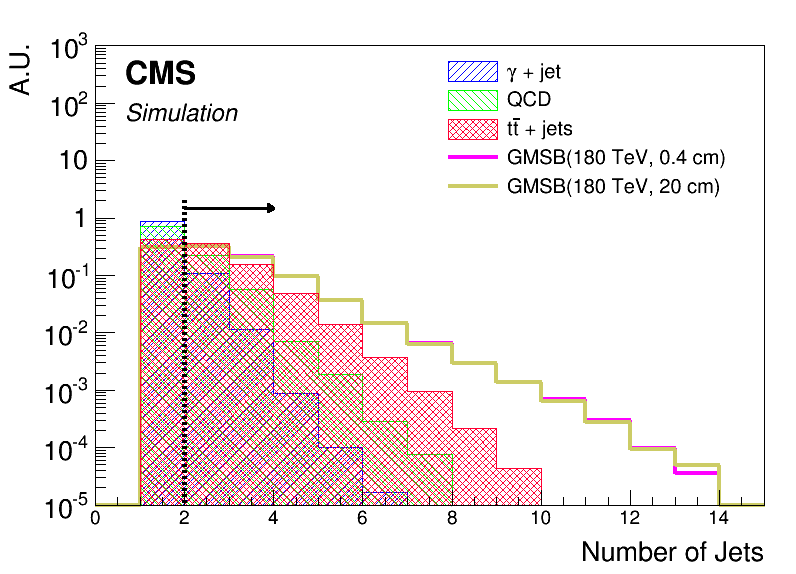
\includegraphics[width=\textwidth]{n-1nJetsMC.png}
\end{column}
\end{columns}
\end{frame}

\subsection{$E^{miss}_T$ Selection}
\begin{frame}
\frametitle{\insertsection: \insertsubsection}
\vspace{-2mm}
\begin{columns}
\begin{column}{5cm}
\begin{footnotesize}
\begin{block}{}
\begin{itemize}
\item Use PF $E^{miss}_T$
\item Apply clean-up filters to remove events with anomalous $E^{miss}_T$ values in both MC and data \href{https://twiki.cern.ch/twiki/bin/viewauth/CMS/MissingETOptionalFilters}{(TWIKI)}
\end{itemize}
\end{block}
\end{footnotesize}
\end{column}
\begin{column}{6cm}
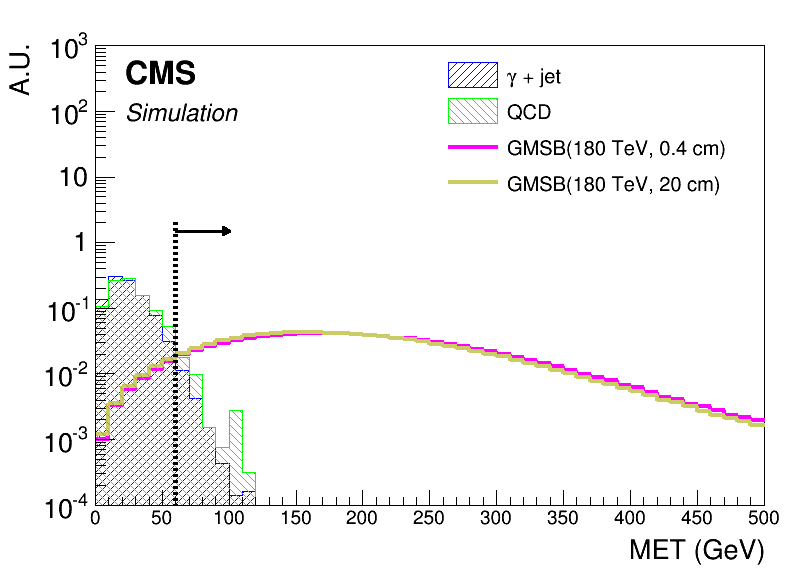
\includegraphics[width=\textwidth]{n-1METMC.png}
\end{column}
\end{columns}

\begin{block}{$E^{miss}_T$ Recommended Filters}
\begin{footnotesize}
\vspace{-4mm}
\begin{columns}
\begin{column}{4.5cm}
\begin{itemize}
\item At least one primary vertex
\item Beam scraping events
\item HBHE noise filter
\item CSC beam halo filter
\item Tracking failure filter
\end{itemize}
\end{column}
\begin{column}{5.5cm}
\begin{itemize}
\item ECAL/HCAL laser events
\item EE bad supercrystal filter
\item ECAL dead cell trigger primitive filter
\item ECAL laser correction filter
\item Anomalous $\rho > 40$.
\end{itemize}
\end{column}
\end{columns}
\end{footnotesize}
\end{block}

\end{frame}




\section[Photon Conv. Meth.]{Photon Conversion Method}
\subsection{first}
\begin{frame}
\frametitle{\insertsection}
\vspace{-5mm}
\begin{columns}
\begin{column}{6.5cm}
\begin{block}{}
\begin{itemize}
%\begin{footnotesize}
%\item Tracker has a large material budget.
\item Up to 60\% of photons traversing CMS tracker can convert into $e^+e^--$pairs
\vspace{2mm}
\item Nuisance in event reconstruction for many physics analyses
\vspace{2mm}
\item \textbf{Photon conversions} to $e^+ e^-$ pairs can be used to obtain the \underline{photon direction}
\vspace{2mm}
\item \textbf{\textcolor{red}{Extrapolate to calculate transverse impact parameter ($d_{XY}$)}}
\vspace{2mm}
\item \textbf{\textcolor{red}{Search for excess using the tail of the $d_{XY}$}}
%\item Photon conversions $\rightarrow$ small opening angle.
%\setbeamertemplate{itemize items}[default]
%\begin{itemize}
%\begin{footnotesize}
%\item $e^+ e^-$ tracks required to be parallel in momentum.
%\item Transverse Impact Parameter (IP) $d_{XY}$: distance of closest approach of photon trajectory to \textbf{\textcolor{red}{beam axis}}.
%\end{footnotesize}
%\end{itemize}
%\end{footnotesize}
\end{itemize}
\end{block}
\end{column}
\begin{column}{5.6cm}
\begin{center}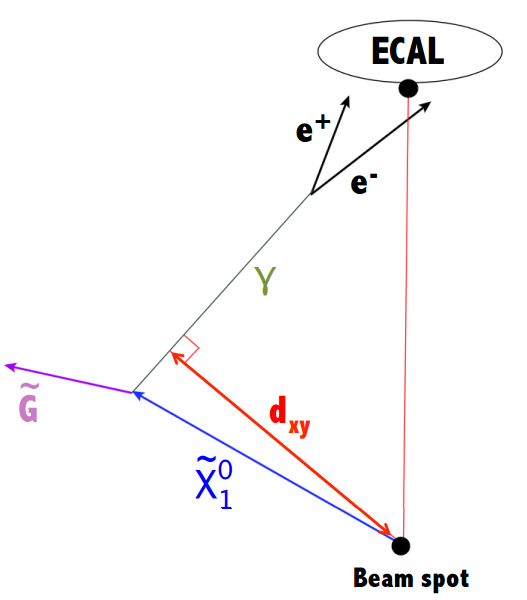
\includegraphics[width=0.65\textwidth]{conversion.png}\\\end{center}
\vspace{-3mm}
\begin{center}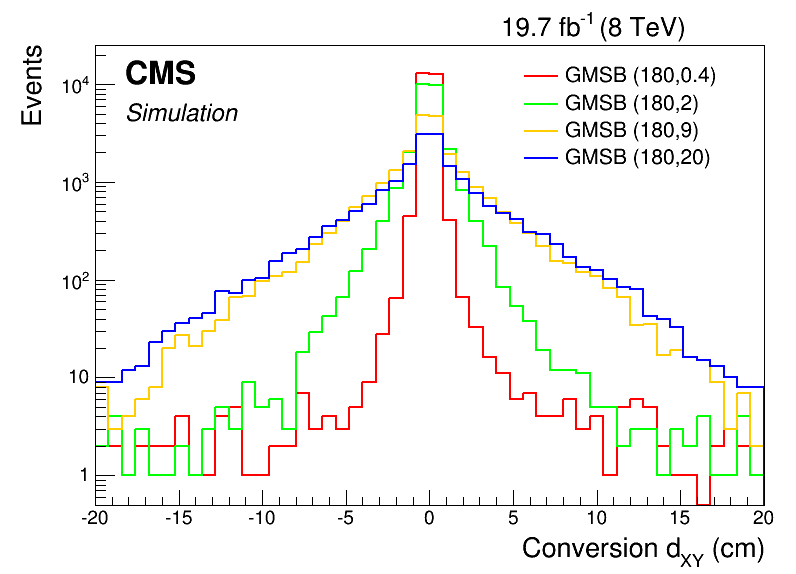
\includegraphics[width=0.89\textwidth]{dxycomparisonsignal.png}\end{center}
\end{column}
\end{columns} 
\end{frame}

\begin{frame}
\label{convselec}
\frametitle{\insertsection}
\vspace{-3mm}
\begin{block}{Conversion Selection}
\begin{itemize}
\item Two oppositely signed tracks;
\item Both need at least five valid hits;
\item Conversion vertex requires valid fit with $\chi^2$ prob. $> 0.01$;
\item Have blessing from EGamma POG \href{https://indico.cern.ch/event/366543/}{ \textcolor{Red}{\textbf{ (Click here for talk) }}}

\end{itemize}
\end{block}
\vspace{-3mm}
\begin{columns}
\begin{column}{6cm}
\begin{center}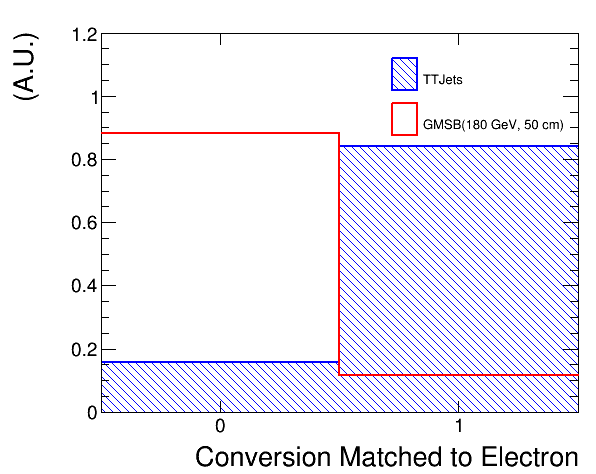
\includegraphics[width=0.78\textwidth]{convmatchedele.png}\\\end{center}
\vspace{-5mm}
\begin{center}Veto conversions found within a $\Delta R$ of 0.25 of a GSF electron.\end{center}
\end{column}
\begin{column}{6cm}
\begin{center}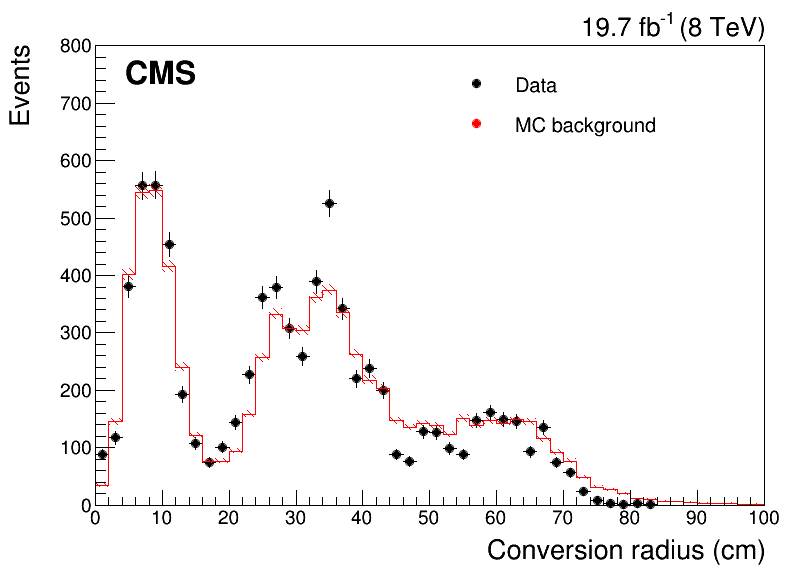
\includegraphics[width=0.85\textwidth]{convRbkgMCstep1.png}\\\end{center}
\vspace{-5mm}
\begin{center}Radius of converted photons to show tracker structure.\end{center}
\end{column}
\end{columns}
\end{frame}


\section[Event Sel.]{Event Selection}

\begin{frame}
\frametitle{\insertsection}
\vspace{-2mm}

\begin{exampleblock}{\footnotesize Signal Region Definition (Feynman diagram, slide \ref{introdu})}
\begin{itemize}
\begin{small}
\item At least 2 photons ($p_T >$ 50 GeV) with leading photon of $p_T > 85$ GeV.
\item At least 2 jets ($p_T >$  35 GeV).
\item At least one photon conversion 
\item $E^{miss}_T > $ 60 GeV (see slide \ref{METoptimisation}).
\end{small}
\end{itemize}
\end{exampleblock}

\begin{block}{\footnotesize Our Backgrounds}
\begin{itemize}
\begin{small}
\item $\gamma$ + jets: real energetic photons \begin{scriptsize}(\textbf{Dominant}: estimate using data)\end{scriptsize}.
\item QCD: jets misidentified as photons \begin{scriptsize}(\textbf{Negligible}: estimate using data)\end{scriptsize}.
\item TTJet: electrons misidentified as photons \begin{scriptsize}(\textbf{Negligible})\end{scriptsize}.
\end{small}
\end{itemize}
\end{block}

\end{frame}


\section[Bkg Est]{Background Estimation}
\subsection{Method}
\begin{frame}
\frametitle{\insertsection}
\begin{columns}
\begin{column}{6cm}
\begin{block}{}
\begin{itemize}
\item Expect bkg to be rich in $\gamma+$jets.
%\vspace{1mm}
\item Instrumental $E^{miss}_T$ will give rise to \textbf{low} $\mathbf{E^{miss}_T}$ distribution.
%\vspace{1mm}
%\item Use 7 TeV estimation method
\vspace{1mm}
\item \textbf{\textcolor{red}{Select events in data with $E^{miss}_T < 30$ but satisfy all other signal selection criteria (to derive shape).}}
\vspace{1mm}
\setbeamertemplate{itemize items}[ball]
\item \textbf{\textcolor{red}{Normalise shape to the $d_{XY}$ peak of data (first bin).}}
\vspace{1mm}
\item \textbf{\textcolor{red}{Fully data driven method}}
\end{itemize}
\end{block}
\end{column}
\begin{column}{6cm}
\begin{center}
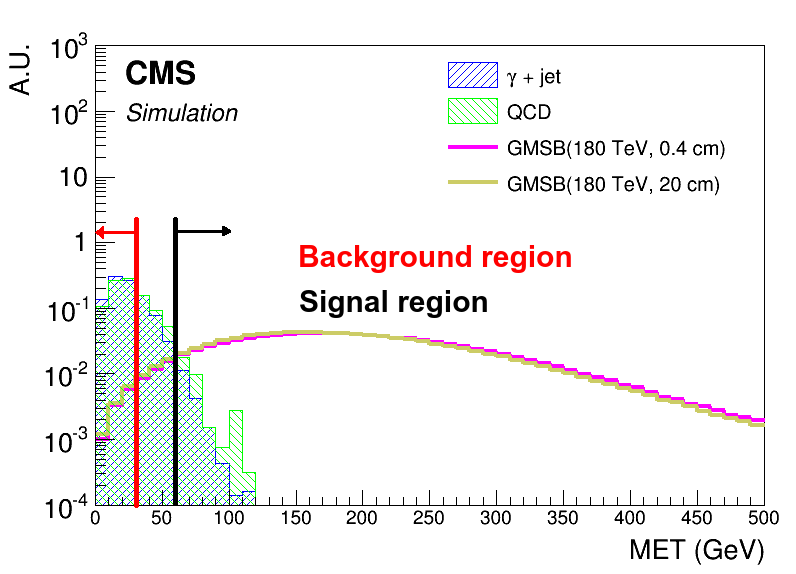
\includegraphics[width=0.9\textwidth]{n-1METMClines.png}
\end{center}
\end{column}
\end{columns}
\end{frame}


\subsection{CR}
\begin{frame}
\label{shapeuncertainty}
\frametitle{\insertsection} 
\begin{columns}
\begin{column}{12cm}
\vspace{-8mm}
\begin{table}
%\caption*{\textbf{EXO-14-017: Table 1}}
\begin{tabular}{l|l|c}
\hline
\hline
Region &  $E^{miss}_T$ requirement  & Photon passes all isolation \\
& & requirements \\
\hline
 \textcolor{Dandelion}{\textbf{CR1}}  &   \textcolor{Dandelion}{\textbf{$\leq 30$ GeV}}        &  \textcolor{Dandelion}{\textbf{Yes}} \\
 CR2  &   $\leq 30$ GeV        &  No \\
 CR3  &   $\geq 60$ GeV        &  No \\
\hline
\hline
\end{tabular}
\end{table}

\end{column}
\end{columns}

\begin{columns}
\begin{column}{5.8cm}
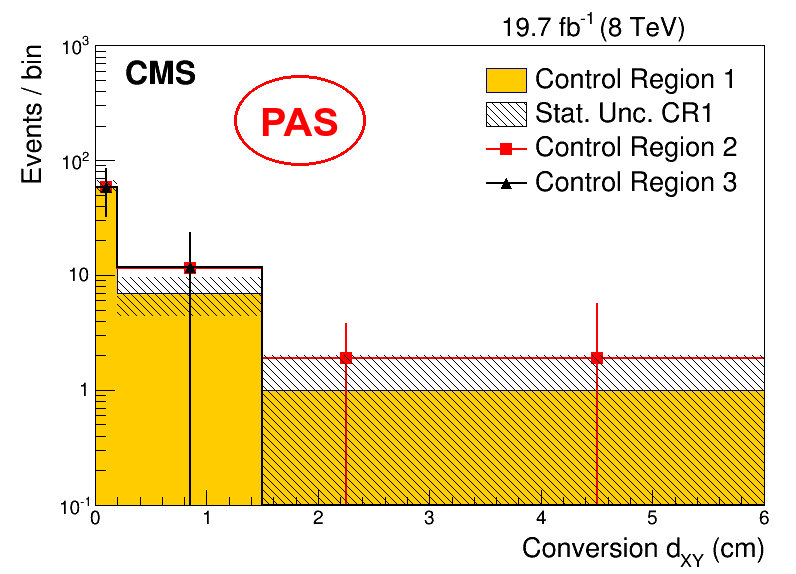
\includegraphics[width=0.97\textwidth]{dxycomparisonfakehighfakelowisolow.png}
\end{column}
\begin{column}{6.5cm}
\setbeamertemplate{itemize items}[ball]
\begin{itemize}
\item \textcolor{Dandelion}{\textbf{CR 1 is nominal bkg. estimate}}
\vspace{1mm}
\item \textbf{All 3 histograms (left) are data}
\vspace{1mm}
\item \textbf{Good agreement between 3 CRs} 
\item \textbf{Signal contam. in CR1 $\leq 1\%$}
\vspace{1mm}
\item \textbf{Use CR 2 as shape systematic} 
\end{itemize}
\end{column}
\end{columns}
\end{frame}


\section{Closure tests for bkg. determination}
\begin{frame}
\frametitle{\insertsection}
\vspace{-2mm}
\begin{center}
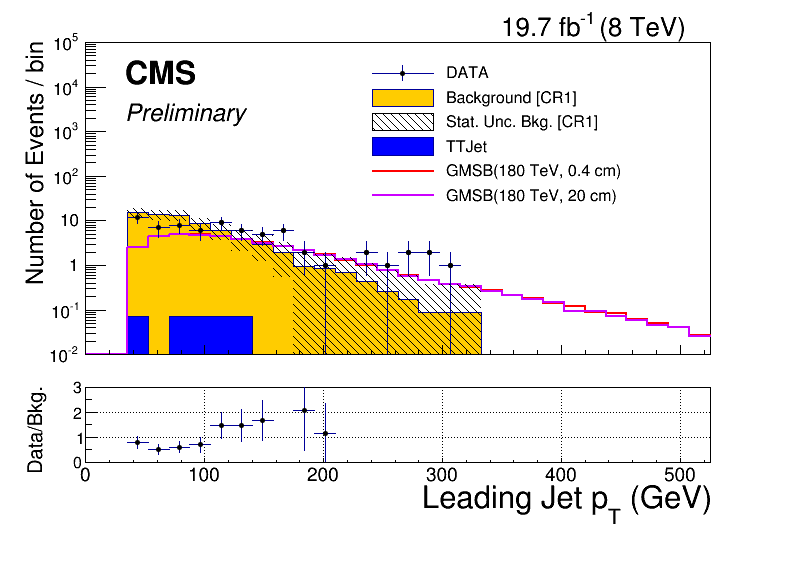
\includegraphics[width=0.48\textwidth]{jetPtDD.png}
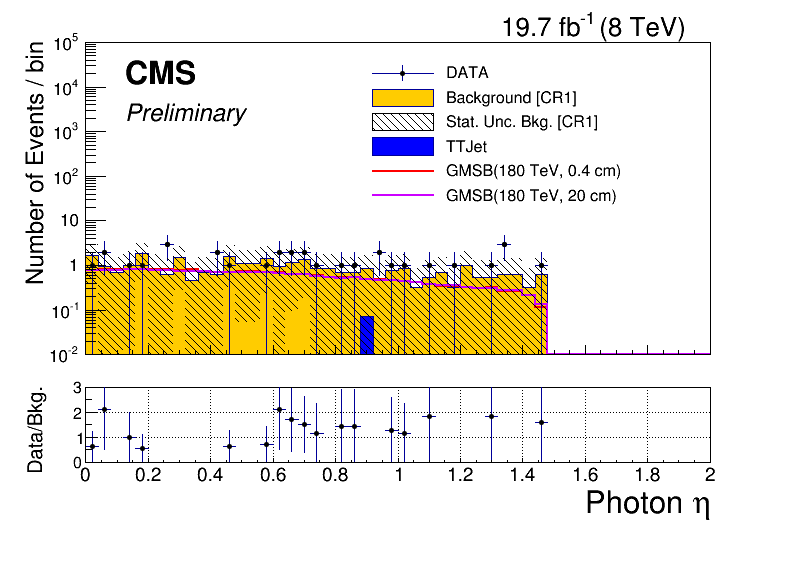
\includegraphics[width=0.48\textwidth]{etaDD.png}\\
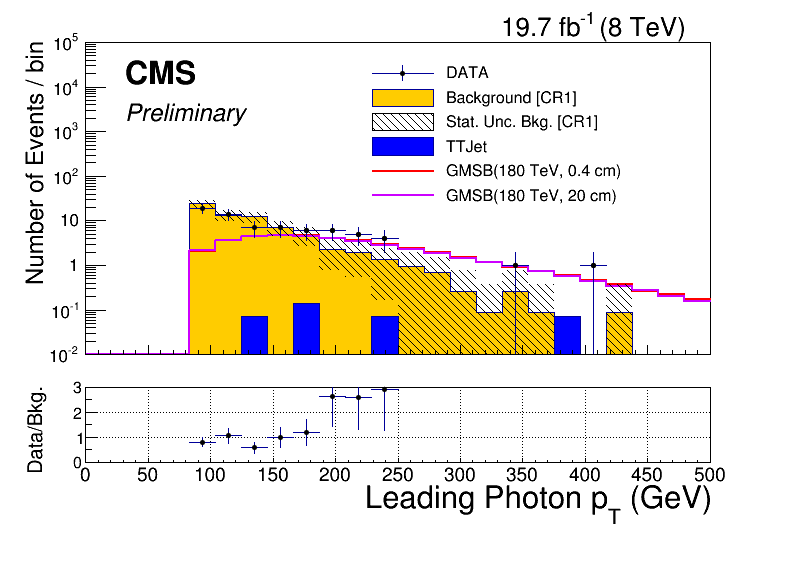
\includegraphics[width=0.48\textwidth]{photPtDD.png}
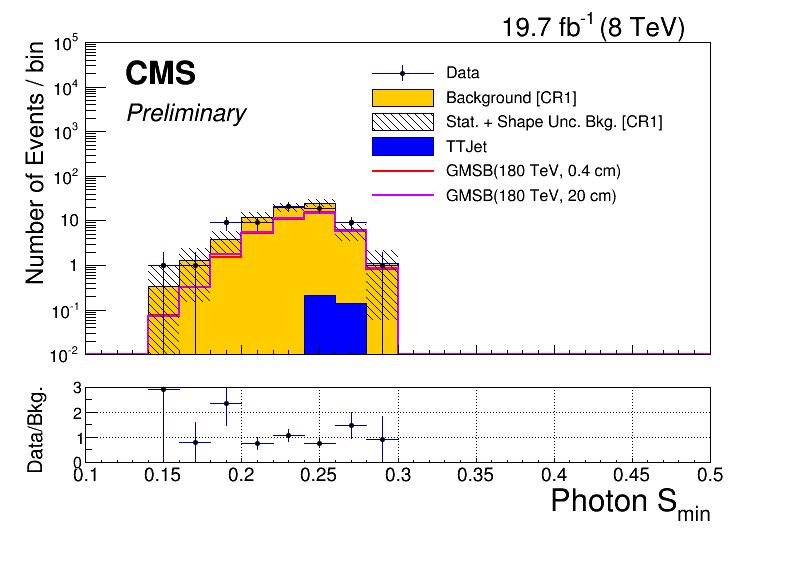
\includegraphics[width=0.48\textwidth]{sMinDD.png}
\end{center}
\end{frame}

\section[MET]{MET optimisation}
\begin{frame}
\frametitle{\insertsection}
\label{METoptimisation}
\begin{columns}
\begin{column}{6cm}
\begin{figure}
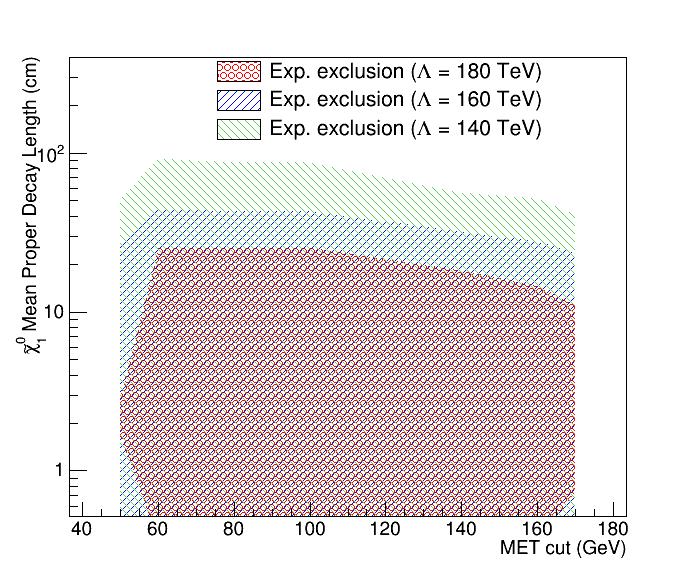
\includegraphics[width=\textwidth]{METoptimisation_noline.png}
\end{figure}
\end{column}
\hspace{-14mm}
\begin{column}{6cm}
\begin{itemize}

\item \textcolor{Black}{\textbf{Can see from slide 15 that signal peaks at high $E^{miss}_T$ while bkg. drops off sharply}}
\vspace{2mm}
\item \textcolor{Black}{\textbf{Pick optimal $E^{miss}_T$ cut by maximising expected exclusion area @95\% C.L.}}
\vspace{2mm}
\item \textcolor{Orange}{\textbf{Input all signal points, data driven bkg. est, final systematics into CLs}}
\vspace{2mm}
\item \textcolor{Orange}{\textbf{See from plot (left) that $E^{miss}_T > 60$ GeV is optimal}}

\end{itemize}
\end{column}
\end{columns}
\end{frame}


\begin{frame}
\frametitle{\insertsection}
\label{METoptimisation}
\begin{columns}
\begin{column}{6cm}
\begin{figure}
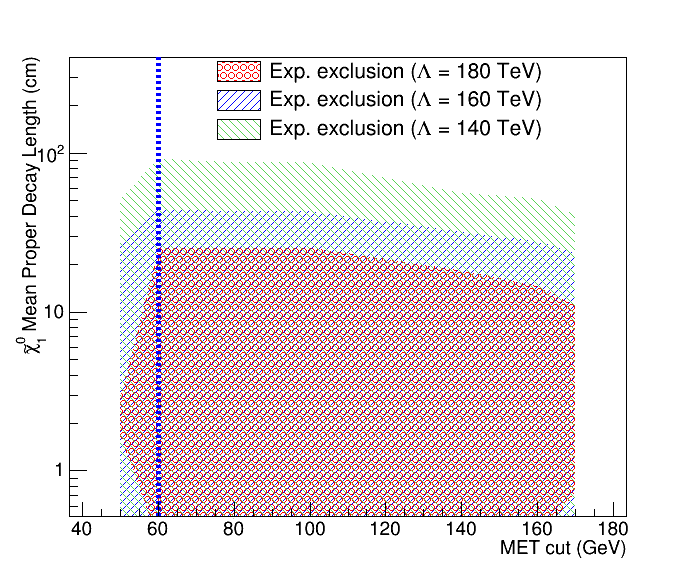
\includegraphics[width=\textwidth]{METoptimisation.png}
\end{figure}
\end{column}
\hspace{-14mm}
\begin{column}{6cm}
\begin{itemize}
\item \textcolor{Black}{\textbf{Can see from slide 15 that signal peaks at high $E^{miss}_T$ while bkg. drops off sharply}}
\vspace{2mm}
\item \textcolor{Black}{\textbf{Pick optimal $E^{miss}_T$ cut by maximising expected exclusion area @95\% C.L.}}
\vspace{2mm}
\item \textcolor{Orange}{\textbf{Input all signal points, data driven bkg. est, final systematics into CLs}}
\vspace{2mm}
\item \textcolor{Orange}{\textbf{See from plot (left) that $E^{miss}_T > 60$ GeV is optimal}}
\end{itemize}
\end{column}
\end{columns}
\end{frame}



\section{Results}

\begin{frame}
\label{dxyhistogram}
\frametitle{\insertsection}
\begin{center}\textbf{Use shape of $d_{XY}$ to search for excess of signal/expected bkg}\end{center}
\begin{center}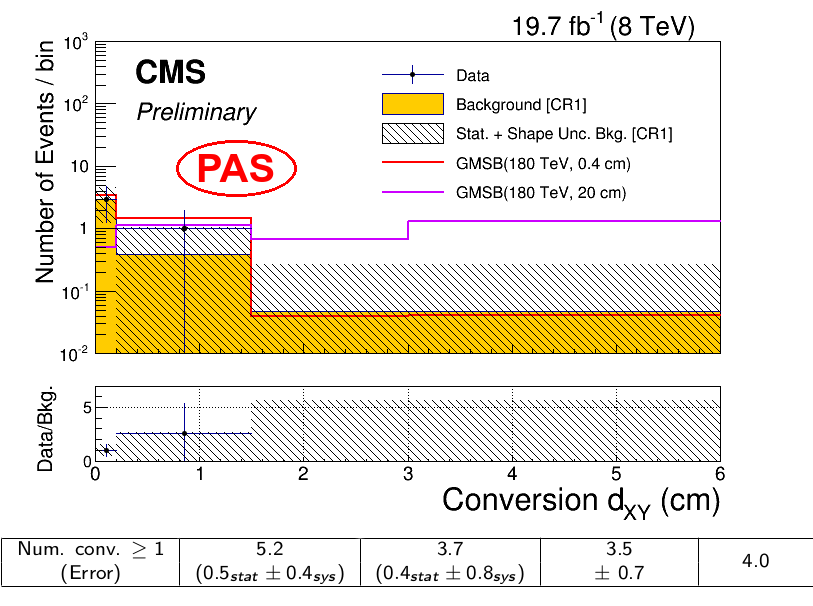
\includegraphics[width=0.8\textwidth]{dXYDD_withtable.png}\end{center}

\end{frame}



%\begin{frame}
%\frametitle{\insertsection: \insertsubsection}
%\begin{scriptsize}
%\vspace{-6mm}
%\begin{columns}
%\begin{column}{9.5cm}
%\begin{table}[h]
%\centering
%\caption*{\textbf{EXO-14-017: Table 3}}
%\begin{tabular}{|c|c|c|c|c|}
%\hline
%\hline
%& GMSB    & GMSB                        & SM bkg. & \multirow{2}{*}{Data} \\
%& (180, 0.4) & (180, 20)        &  estimate(CR1)           &  \\
%\hline
%All &                                   285                &285  & - & 5.21e+11\\
%Preselection &                  182                &176  & - & 7.34e+10\\
%$E^{miss}_T > $ 60 &    174                &167  & - & 1.86e+09\\
%Num. jets  $\geq$ 2 &   102                &98   & - & 4.55e+08\\
%Num. phot. $\geq$ 2 &   41                 &41   & - & 1.42e+06\\
%&&&&\\
%Num. conv. $\geq$ 1 &   5.2 $\pm \ 0.5$  &3.7 $\pm \ 0.8$ & 3.5 $\pm \ 0.7$ & 4.0\\
%\hline
%\hline
%\end{tabular}
%\label{table:cutflow}
%\end{table}

%\end{column}
%\end{columns}
%\end{scriptsize}
%\begin{itemize}
%\item Preselection: 
%\begin{itemize}
%\setbeamertemplate{itemize items}[default]
%\item Passing the trigger
%\item At least one good reconstructed vertex
%\item At least one loosely identified photon
%\end{itemize}
%\setbeamertemplate{itemize items}[ball]
%\end{itemize}
%\end{frame}





\section[Unct.]{Uncertainties}

\begin{frame}
\frametitle{\insertsection}
\begin{exampleblock}{Signal (same as EXO-11-067)}
\begin{itemize}
\item Luminosity (2.6 \%)
\item Jet Energy Scale
\setbeamertemplate{itemize items}[default]
\begin{itemize}
\item Use official recommendation from JetMET POG.
\end{itemize}
\setbeamertemplate{itemize items}[ball]
\item Photon Energy Scale 
\setbeamertemplate{itemize items}[default]
\begin{itemize}
\item 0.6\% variation on photon $p_T$.
\end{itemize}
\setbeamertemplate{itemize items}[ball]
\item Conversion Reconstruction Efficiency \textcolor{blue}{(largest/see slide \ref{convrecoeff})}
\item Statistical
\end{itemize}
\end{exampleblock}
\begin{alertblock}{Background}
\begin{itemize}
\item Background shape uncertainty (slide \ref{shapeuncertainty})
\item Statistical
\end{itemize}
\end{alertblock}
\end{frame}

\subsection{Conversion Reconstruction Efficiency}
\begin{frame}
\frametitle{\insertsection: \insertsubsection}
\begin{alertblock}{}
\begin{itemize}
\item Method is to sum in quadrature the effect of two things:
\setbeamertemplate{itemize items}[default]
\begin{enumerate}
\item Difference between data and MC in $Z \rightarrow \mu \mu \gamma$ events.
\item Difference between $Z \rightarrow \mu \mu \gamma$ and GMSB MC.
%\item Sum these numbers in quadrature.
\end{enumerate}
\end{itemize}
\end{alertblock}
\setbeamertemplate{itemize items}[ball]
%\begin{block}{}
\begin{itemize}
\item Use $Z \rightarrow \mu \mu \gamma$ data and MC control studies
\item Use results from Nancy Marinelli et al. \\ 
(\href{http://cms.cern.ch/iCMS/analysisadmin/cadilines?line=EGM-14-001}{EGM-14-001} and \href{https://indico.cern.ch/event/292932/contribution/1/material/slides/1.pdf}{Approval Talk}).
\item Conversion prob. $\times$ reconstruction eff. = $\frac{\# \ \textrm{of conversions}}{\# \ \textrm{of photons}}$
\end{itemize}
%\end{block}
\begin{table}
\begin{tabular}{|c|c|c|c|c|}
\hline
& conversions & photons & Eff. (\%) & Data-MC scale factor\\
\hline
data & 5560 & 70209 & 7.9 $\pm$ 0.14 & \multirow{2}{*}{0.93 $\pm 0.03$}\\
MC & 5742 & 67653 & 8.5 $\pm$ 0.15 & \\
\hline
\end{tabular}
\end{table}
\vspace{3mm}
\end{frame}

\begin{frame}
\frametitle{\insertsection: \insertsubsection}
\begin{columns}
\begin{column}{7.4cm}
\begin{itemize}
\item GMSB samples also have certain conv. prob. $\times$ rec. eff. (see figure).
\item Differs from $Z \rightarrow \mu \mu \gamma$ conv. prob. $\times$ rec. eff. (previous slide).
\item Ratio accounts for extra scale factor. 
\item This scale factor, together with the Data-MC scale factor makes up our systematic uncertainty.
\item Example: \textcolor{green}{GMSB (180 TeV, 9 cm)}
\end{itemize}
\end{column}
\begin{column}{5cm}
\begin{figure}
\centering
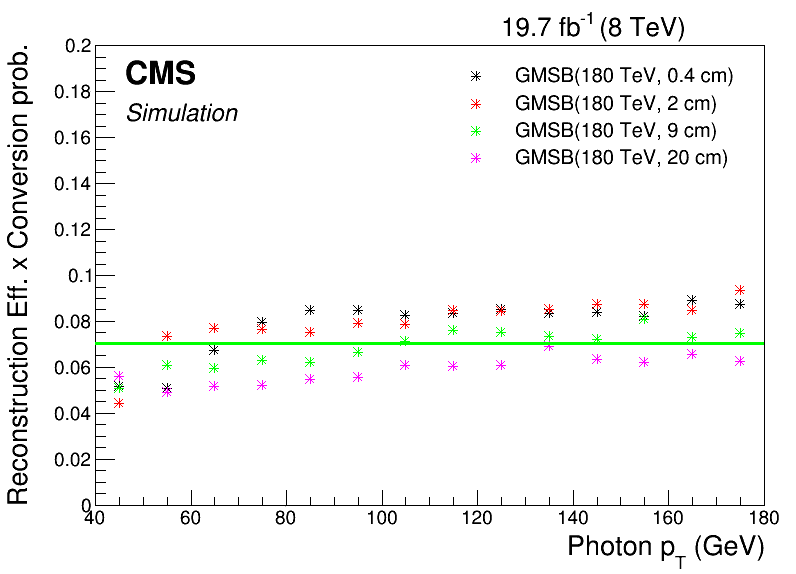
\includegraphics[width=\textwidth]{dxyefficiencyL180.png}
\end{figure}
\end{column}
\end{columns}
\vspace{3mm}
\begin{center}
$0.19 = \sqrt{(1-0.93)^2 + \left(1-\frac{\textcolor{green}{7.2\%}}{8.5\%}\right)^2}$
\end{center}
\end{frame}


\begin{frame}
\label{convrecoeff}
\label{signaluncert}
\frametitle{\insertsection: Final Values}
\begin{itemize}
\item From \href{http://cms.cern.ch/iCMS/analysisadmin/cadilines?line=EXO-11-067}{EXO-11-067} we expected the conversion reconstruction efficiency to be dominant.
%\item Computed most other uncertainties they mention.
\item Exact values depend on which signal point is considered. Table below shows full range.
\end{itemize}
\begin{table}
\centering
\begin{tabular}{c c||c|}
\cline{2-3}
\multicolumn{1}{c|}{}& Source & Uncertainty (\%) \\ \hline
\hline
\multicolumn{1}{|c|}{\multirow{5}{*}{Signal}} & Conversion reconstruction efficiency & $7-45$ \\
\multicolumn{1}{|c|}{} & Integrated luminosity & 2.6\\
\multicolumn{1}{|c|}{}& Jet energy scale & $< 1$\\
\multicolumn{1}{|c|}{}& Photon energy scale & $< 1$\\
\multicolumn{1}{|c|}{}& Statistical & $<1$\\ \hline
\multicolumn{1}{|c|}{\multirow{2}{*}{Background}} & Shape & CR2 \\
\multicolumn{1}{|c|}{}& Statistical & 13\\
\hline
\end{tabular}
\end{table}
\end{frame}



\section{Upper Limits}
\begin{frame}
\label{explimits}
\frametitle{\insertsection: \insertsubsection}
\vspace{-3mm}
\begin{columns}
\begin{column}{3.8cm}
\begin{block}{$\Lambda = 140$ TeV}
\begin{center}
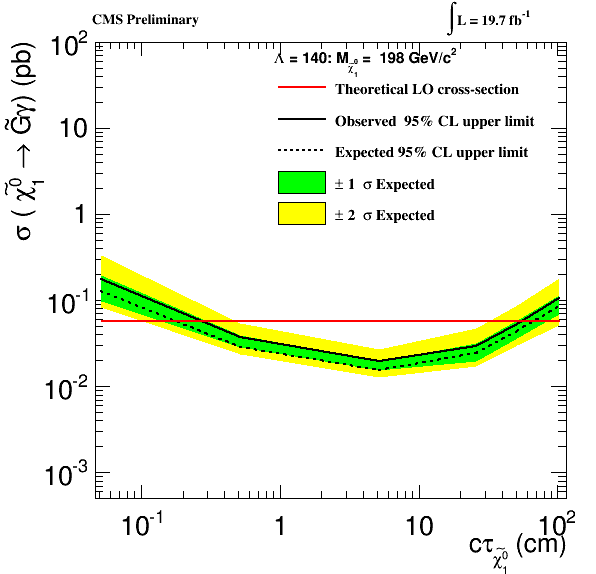
\includegraphics[width=\textwidth]{exclusion_limit_L140_FullCLs.png}
\end{center}
\end{block}
\end{column}
\begin{column}{3.8cm}
\begin{block}{$\Lambda = 160$ TeV}
\begin{center}
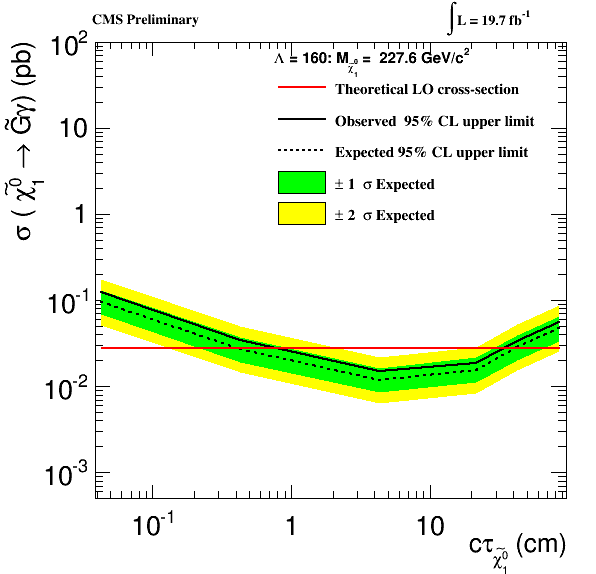
\includegraphics[width=\textwidth]{exclusion_limit_L160_FullCLs.png}
\end{center}
\end{block}
\end{column}
\begin{column}{3.8cm}
\begin{block}{$\Lambda = 180$ TeV}
\begin{center}
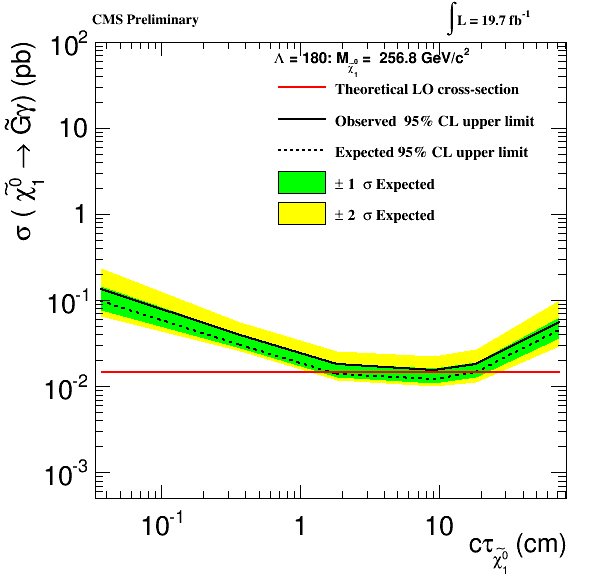
\includegraphics[width=\textwidth]{exclusion_limit_L180_FullCLs.png}
\end{center}
\end{block}
\end{column}
\end{columns}
\begin{columns}
\begin{column}{7.5cm}
\end{column}
\end{columns}
\begin{itemize}
\begin{small}
\setbeamertemplate{itemize items}[ball]
\item Calculate ULs using CLs (10,000 toys) %input histograms from slide \ref{dxyhistogram})
\item Shape uncertainty on bkg. (slide \ref{shapeuncertainty}) + uncertainties on the signal (slide \ref{signaluncert})
\item First bin in $d_{XY}$ is excluded from limit computation
\end{small}
\end{itemize}
\end{frame}


\begin{frame}
\frametitle{2D exclusion results}
\begin{center}
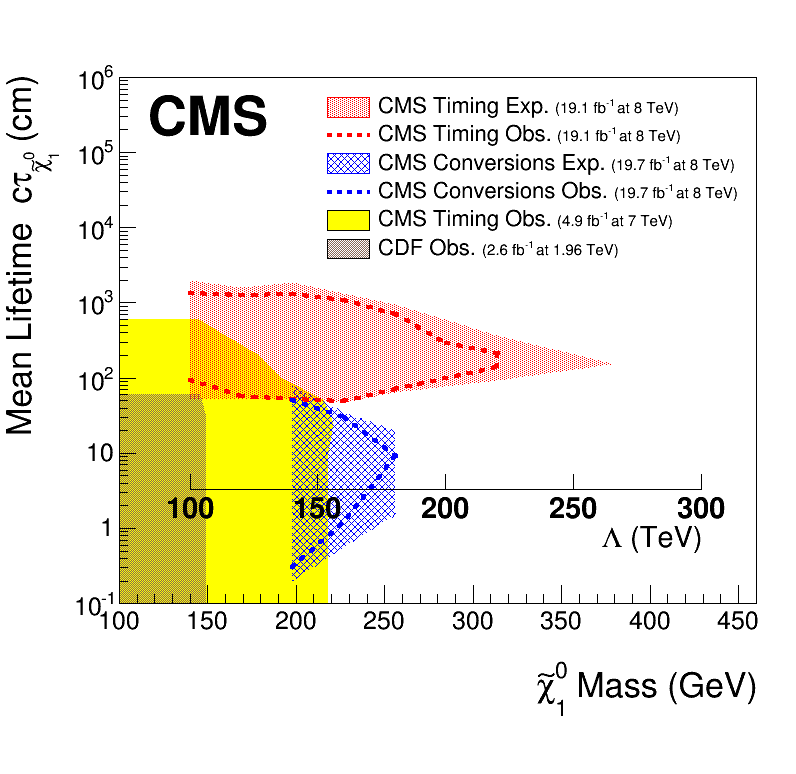
\includegraphics[width=0.75\textwidth]{limit2D_everything.png}
\end{center}

%\begin{itemize}
%\begin{small}
%\item Results from conversions analysis helps to exclude low c$\tau$ region  
%\item Results from EXO-12-035 and this analysis work nicely together 
%\end{small}
%\end{itemize}

\end{frame}


\subsection{Overview for 13 TeV}
\begin{frame}
\frametitle{\insertsubsection}
\begin{columns}
\begin{column}{5.5cm}
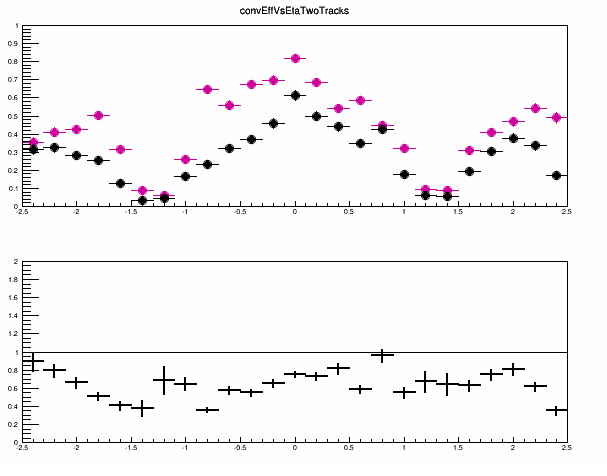
\includegraphics[width=\textwidth]{convtracks.png}
\begin{center}From Nancy Marinelli\end{center}
\end{column}
\hspace{-8mm}
\begin{column}{7.2cm}
\begin{itemize}
\begin{small}
\item \textbf{Main issue will be the PU rate.}
\item Conv. rec. eff. should stay unchanged with 10 BX at 25 ns and 20 BX at 50 ns.
\item Software pre-release validation: check 35 BX at 25 ns and 50 ns.
\setbeamertemplate{itemize items}[default]
\begin{itemize}
\item \textbf{50 ns:} conv. rec. eff. more or less stays the same.
\item \textcolor{red}{\textbf{25 ns:} conv. rec. eff. decreases a lot ($\sim$ 40\% less)}
\item Left plot shows the efficiency a function of $\eta$.
\setbeamertemplate{itemize items}[circle]
\begin{itemize}
\item \textcolor{purple}{10 BX at 25 ns} 
\item 35 BX at 25 ns
\end{itemize}
\end{itemize}
\end{small}
\end{itemize}
\end{column}
\end{columns}
\end{frame}


\section{Summary}
\begin{frame}
\frametitle{Summary}
\begin{itemize}
\item \textcolor{Orange}{\textbf{Performed a search for displaced photons using conversions at 8 TeV}} 

\vspace{3mm}

\item \textcolor{Orange}{\textbf{Analysis keeps the main features from the 7 TeV result}}
\begin{itemize}
\item i.e. Bkg. estimation, systematic assessment, signal samples
\end{itemize}
\vspace{3mm}

\item \textcolor{Orange}{\textbf{But also has added some improvements}} 
\begin{itemize}
\item i.e. Use a full shape analysis instead of cut and count, $E^{miss}_T$ optimisation 
\end{itemize}

\vspace{3mm}

\item \textcolor{Orange}{\textbf{Analysis is complementary to the ECAL timing method}}

\vspace{3mm}

\item \textcolor{Orange}{\textbf{Aiming for approved PAS only}} 
\end{itemize}

\end{frame}





\section[ARC]{ARC Comments}



\begin{frame}
\frametitle{\insertsection}
\begin{center}Do the isolation variables make sense for displaced photons?\end{center}
\begin{columns}
\begin{column}{6cm}
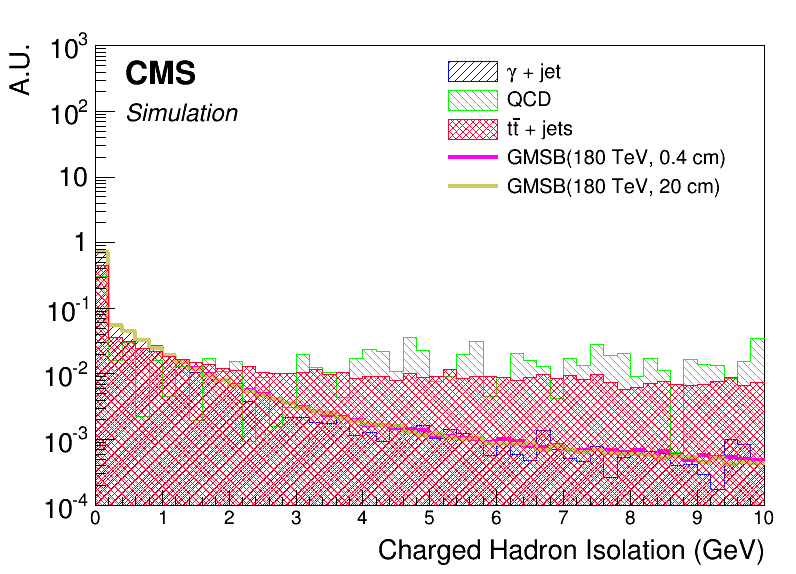
\includegraphics[width=\textwidth]{chadMCrealnocuts.png}
\end{column}
\begin{column}{6.5cm}
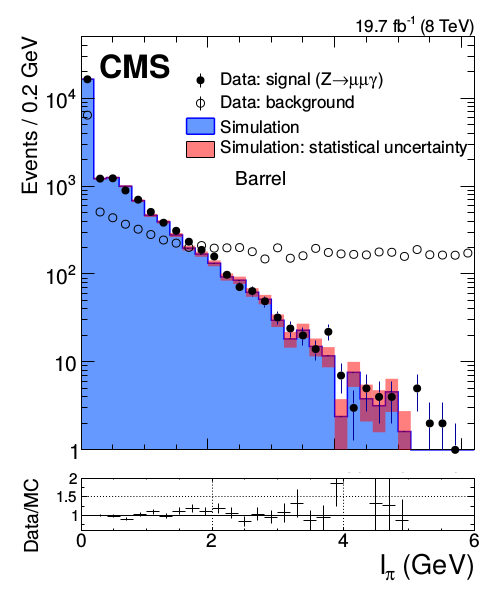
\includegraphics[width=0.8\textwidth]{chadiso_nancy.png}\\
\end{column}
\end{columns}
\begin{center}Matches with plots from EGM-14-001.\end{center}

\end{frame}

\begin{frame}
\frametitle{\insertsection}
\begin{center}Do the isolation variables make sense for displaced photons?\end{center}
\begin{columns}
\begin{column}{6cm}
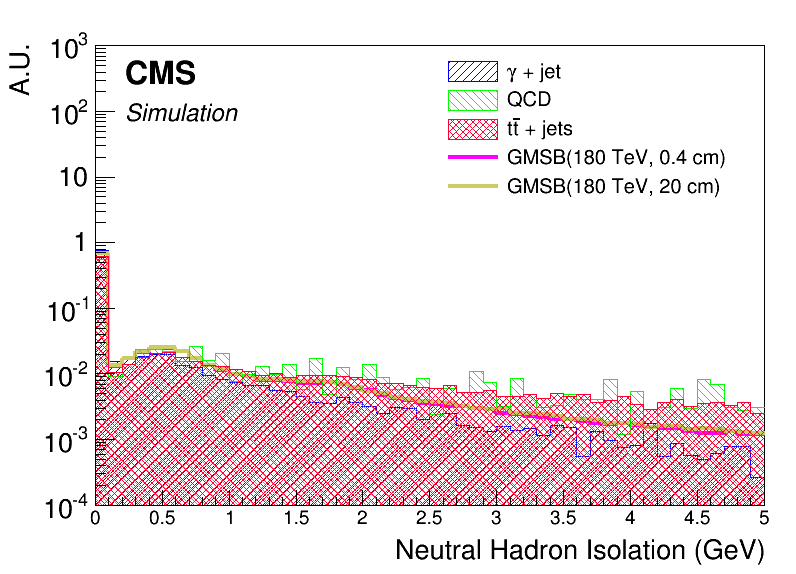
\includegraphics[width=\textwidth]{nhadMCrealnocuts.png}
\end{column}
\begin{column}{6.5cm}
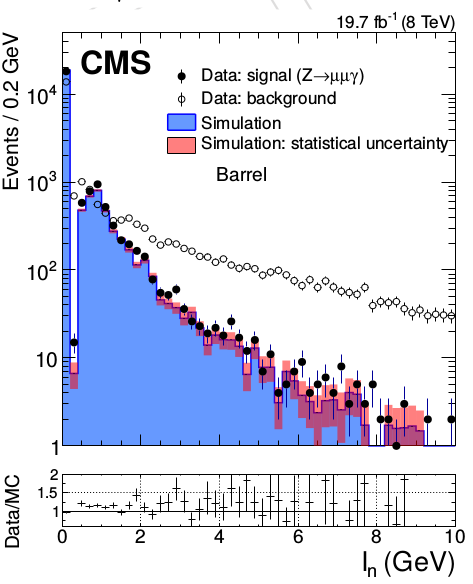
\includegraphics[width=0.8\textwidth]{nhadiso_nancy.png}\\
\end{column}
\end{columns}
\begin{center}Matches with plots from EGM-14-001.\end{center}
\end{frame}

\begin{frame}
\frametitle{\insertsection}
\begin{center}Do the isolation variables make sense for displaced photons?\end{center}
\begin{columns}
\begin{column}{6cm}
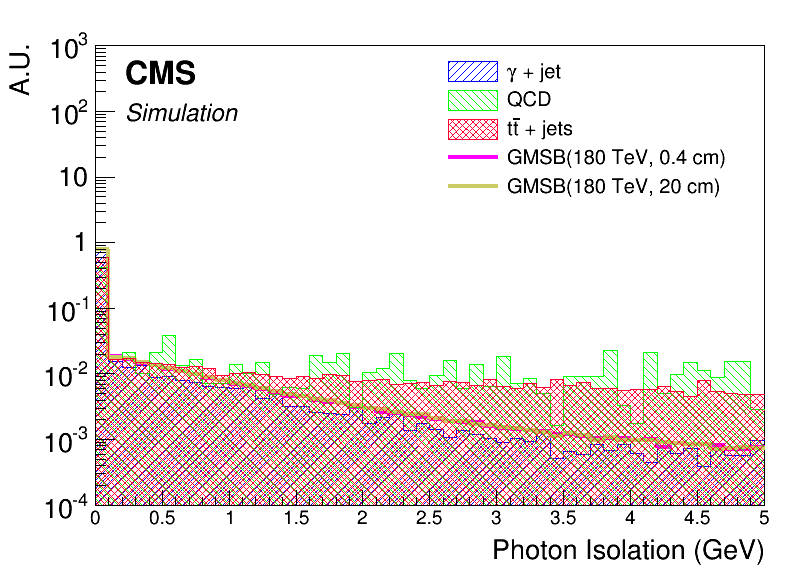
\includegraphics[width=\textwidth]{photisoMCrealnocuts.png}
\end{column}
\begin{column}{6.5cm}
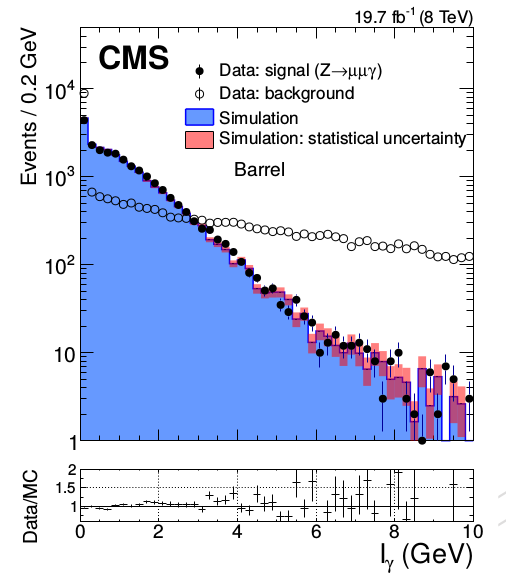
\includegraphics[width=0.8\textwidth]{photiso_nancy.png}\\
\end{column}
\end{columns}
\begin{center}Matches with plots from EGM-14-001.\end{center}
\end{frame}

\begin{frame}
\frametitle{\insertsubsection}

Look at the $p_T$ spectrum of converted and non converted photons. They should be proportional after correcting for the efficiency.

\begin{figure}
\centering
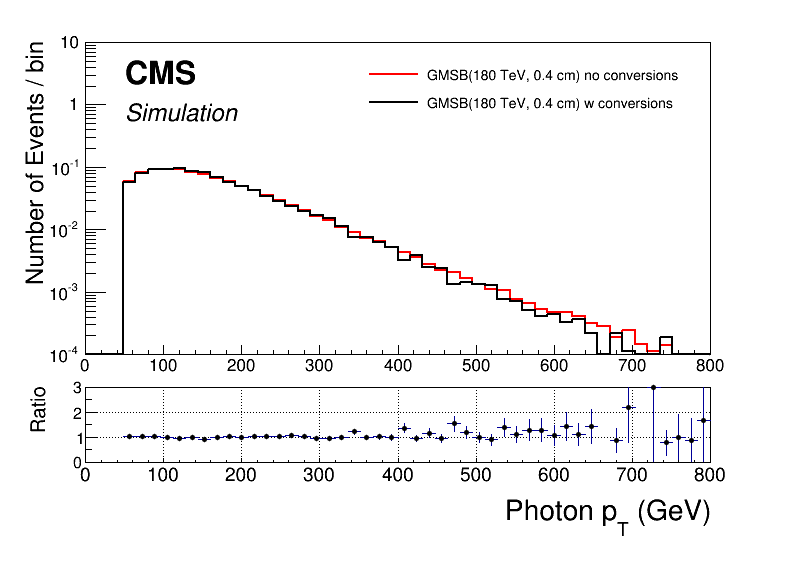
\includegraphics[width=0.8\textwidth]{ptphot.png}
\end{figure}
\end{frame}

\begin{frame}
\frametitle{\insertsection}
\vspace{-3mm}
\begin{center}As sanity check (to see if you are really getting conversions and not random stuff) 
can you try to plot the E taken from ECAL divided by the p measured from the tracks. \end{center}
\begin{center}
\begin{columns}
\begin{column}{7cm}
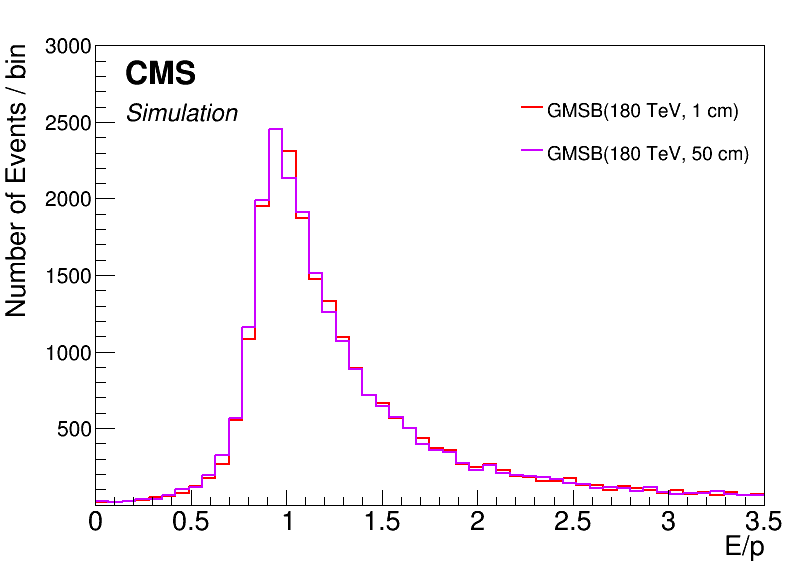
\includegraphics[width=0.8\textwidth]{eoverp.png}
\end{column}
\begin{column}{6.5cm}
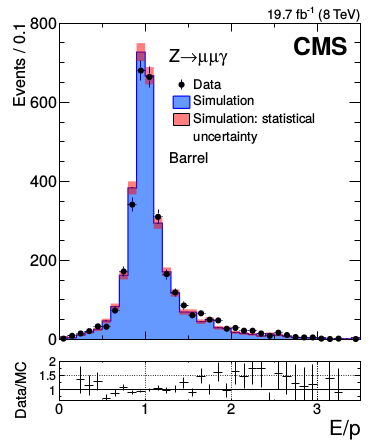
\includegraphics[width=0.7\textwidth]{Eoverp_nancy.png}
\end{column}
\end{columns}
\end{center}
\begin{center}
Agrees with Fig. 13 from EGM-14-001.
\end{center}
\end{frame}

\begin{frame}
\frametitle{\insertsection}
\begin{figure}
\centering
Look at the $R_9$ $(e3x3/E(sc)$ variable for signal photons and compare with the background.
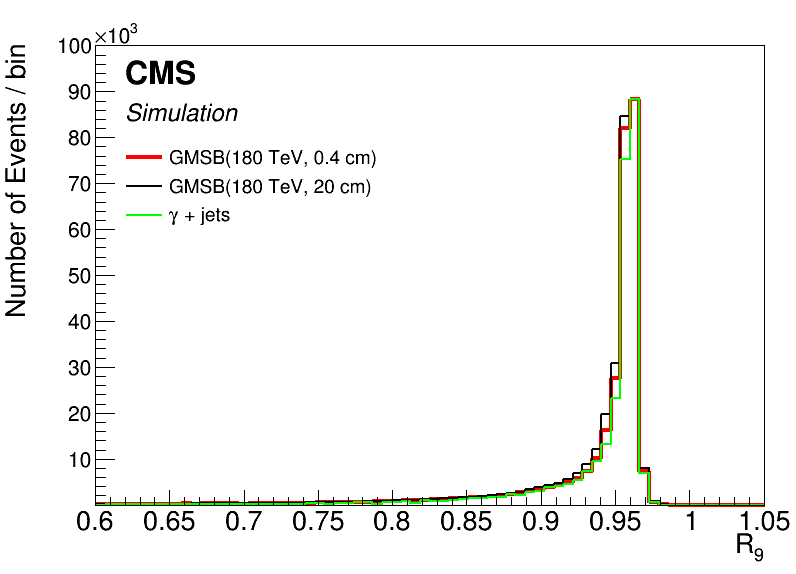
\includegraphics[width=0.55\textwidth]{rninewithandwithoutconversions_GMSBvsGPT.png}
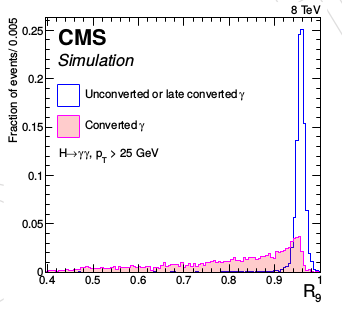
\includegraphics[width=0.45\textwidth]{r9_nancy.png}
\end{figure}
\end{frame}

\begin{frame}
\frametitle{\insertsection}
\begin{center}What is the conversion efficiency in bins of $d_{XY}$?\end{center}
\begin{columns}
\begin{column}{6cm}
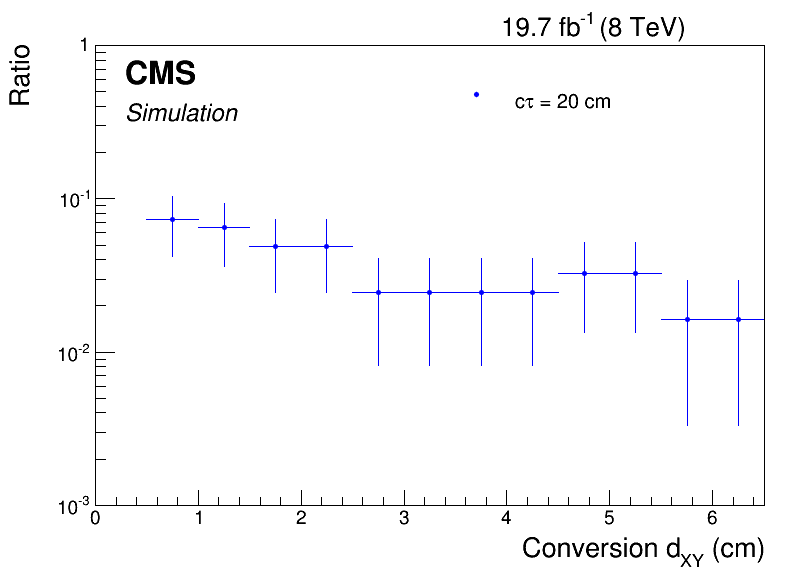
\includegraphics[width=\textwidth]{dxyefficiencygenelectron_loose_convRunder40.png}\\
\end{column}
\hspace{-3mm}
\begin{column}{7cm}
\begin{itemize}
\item Ratio $= \frac{\#(conv. \ RECOed + GENmatch)}{\# (conv. \ GEN)}$
\item Fairly constant up to large $d_{XY}$ in MC
\item Lack large enough data sample to do this for data
\setbeamertemplate{itemize items}[default]
\begin{itemize}
\item Suggestion: look at cosmic data
\item Very few events passing conv. rec. (as expected)
\end{itemize}
\end{itemize}
\end{column}
\end{columns}
\end{frame}


\begin{frame}
\frametitle{\insertsection}
\begin{columns}
\begin{column}{6cm}
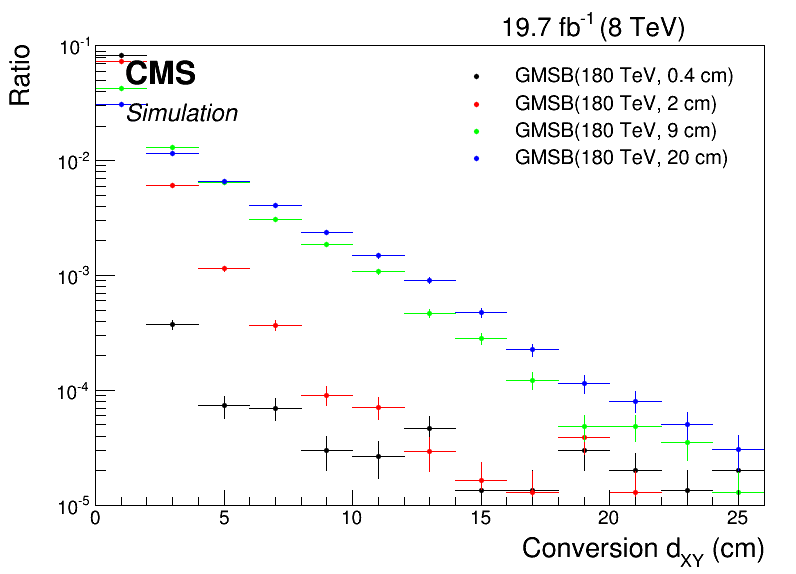
\includegraphics[width=\textwidth]{dxyefficiencyifodxyL180.png}\\
\end{column}
\hspace{-4mm}
\begin{column}{6.77cm}
\begin{itemize}
\item Ratio $= \frac{\# conversions}{\# photons}$
\item Includes conversion probability
\item Main sensitivity is $d_{XY} > \sim 1.5$ cm
\item Probability goes down factor $\sim 5$ when $d_{XY}$ reaches 6 cm
\item Not really necessary to know efficiency at 6 cm
\end{itemize}
\end{column}
\end{columns}
\end{frame}


\begin{frame}
\frametitle{\insertsection: \insertsubsection}
Comparison between cut and count method and shape analysis.
\begin{footnotesize}
\begin{itemize}
\item Cut and count method where a cut at $|d_{XY}|> 1.5$ cm is applied (left).
\item Full shape analysis for $\Lambda = 180$ TeV (right).
\item Both used asymptotic limit setter.
%\item Gain especially visible at low lifetimes ($c\tau$).
\end{itemize}
\end{footnotesize}
\begin{figure}
\centering
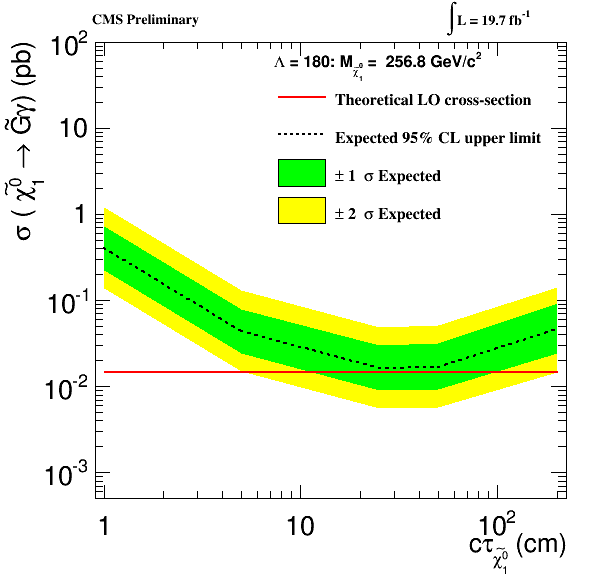
\includegraphics[width=0.5\textwidth]{exclusion_limit_L180_cutandcount.png}
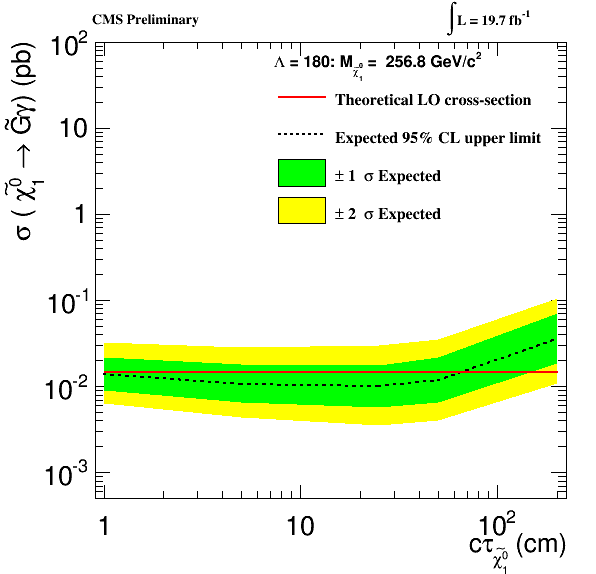
\includegraphics[width=0.5\textwidth]{exclusion_limit_L180_4bins_60gev.png}
\end{figure}
\end{frame}




\begin{frame}
\frametitle{\insertsection}
\begin{center}
\vspace{-3mm}
\begin{scriptsize}
\begin{itemize}
\item Inflated the systematic error on the conv. reco. eff. to show it has zero impact on the limits.
\item We show the exclusion plots using asymptotic CLs in the $\Lambda = 180$ TeV plane. Nominal (upper left), increasing the systematic errors on the signal with 10\% (upper middle), 20\% (upper right), 50\% (lower left), 100\% (lower middle) and 150\% (lower right).
\end{itemize}
\end{scriptsize}
\vspace{3mm}
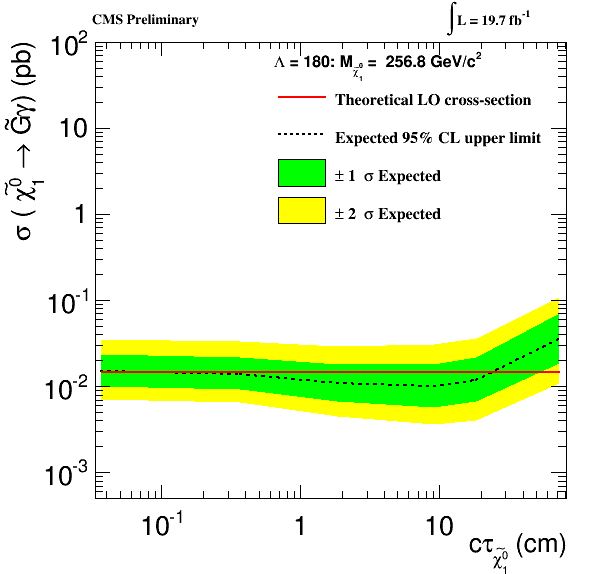
\includegraphics[width=0.25\textwidth]{exclusion_limit_L180.png}
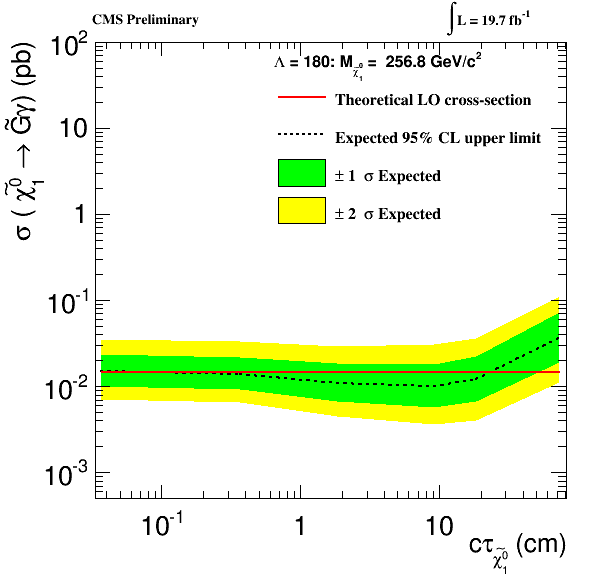
\includegraphics[width=0.25\textwidth]{exclusion_limit_L180_10syst.png}
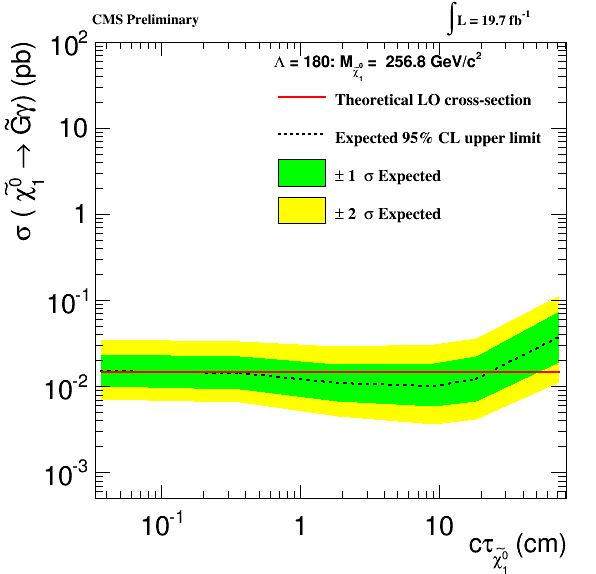
\includegraphics[width=0.25\textwidth]{exclusion_limit_L180_20syst.png}
\\
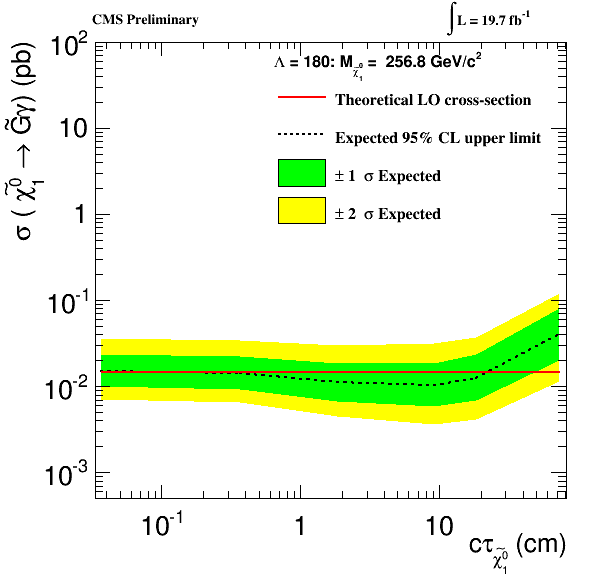
\includegraphics[width=0.25\textwidth]{exclusion_limit_L180_50syst.png}
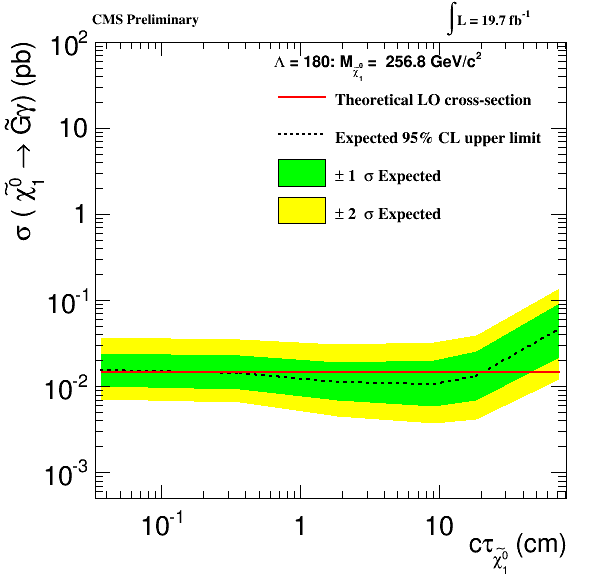
\includegraphics[width=0.25\textwidth]{exclusion_limit_L180_100syst.png}
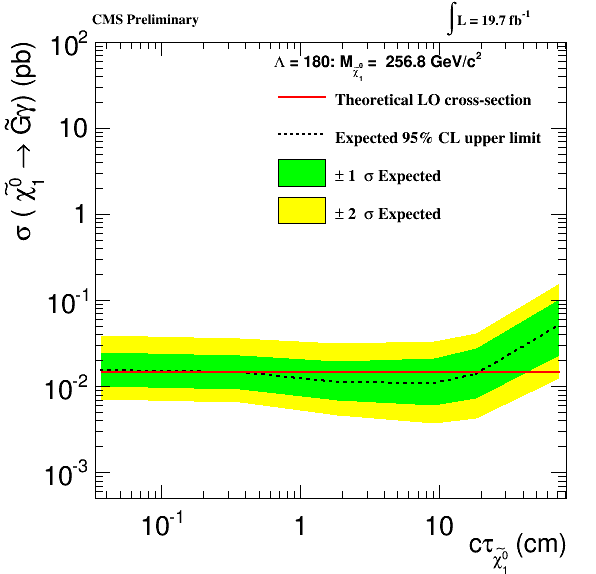
\includegraphics[width=0.25\textwidth]{exclusion_limit_L180_150syst.png}
\end{center}
\end{frame}






\begin{frame}
\Huge
\begin{center}
Thank You
\end{center}
\end{frame}


%\section{}


%\begin{frame}
%\frametitle{Back Up}
%\begin{center}
%\includegraphics[width=0.5\textwidth]{n-1etaMC.png}
%\includegraphics[width=0.5\textwidth]{n-1jetPtMC.png}
%\end{center}
%\end{frame}

%\begin{frame}
%\frametitle{Back Up}
%\begin{center}
%\includegraphics[width=0.5\textwidth]{n-1nPhotMC.png}
%\includegraphics[width=0.5\textwidth]{n-1photPtMC.png}
%\end{center}
%\end{frame}

%\begin{frame}
%\frametitle{Back Up}
%\begin{center}
%\includegraphics[width=0.5\textwidth]{n-1sMinMC.png}
%\includegraphics[width=0.5\textwidth]{n-1sigmaietaMC.png}
%\end{center}
%\end{frame}

%\begin{frame}
%\frametitle{Back Up}
%\begin{center}
%\includegraphics[width=0.8\textwidth]{unnamed.png}
%\end{center}
%\end{frame}


%\begin{frame}
%\frametitle{Back Up}
%\includegraphics[width=\textwidth]{razor.png}
%\end{frame}

%\begin{frame}
%\frametitle{Back Up}
%\includegraphics[width=\textwidth]{rsqrdtriggerL180_subleading55.png}
%\end{frame}


%\begin{frame}
%\frametitle{Back Up}
%\includegraphics[width=\textwidth]{tracker.png}
%\end{frame}

%\begin{frame}
%\frametitle{Back Up}
%\includegraphics[width=\textwidth]{trackingeff.png}
%\end{frame}

%\begin{frame}
%\frametitle{Back Up}
%\begin{center}\includegraphics[width=0.7\textwidth]{Atlas.png}\\\end{center}
%\begin{center}\href{http://arxiv.org/pdf/1409.5542v1.pdf}{Arxiv}\end{center}
%\end{frame}
\end{document}
